\documentclass[12pt, letterpaper]{article}
\usepackage[utf8]{inputenc}
\usepackage[margin=1in]{geometry}
\usepackage[super]{nth}
\usepackage{hyperref}
\usepackage{lineno}
\usepackage[
singlelinecheck=false
]{caption}
\usepackage{amsmath}
\usepackage{bm}
\usepackage{bbm}
\usepackage{graphicx}
\usepackage{csvsimple}
\usepackage[section]{placeins}

\title{Method to infer relatedness using low coverage ancient DNA}
\author{Divya Ratan Popli, Benjamin M. Peter}
\date{5 August 2021}
\linenumbers

\setlength{\parskip}{1em}
\setlength{\parindent}{0em}

\newcommand{\BZ}{\mathbf{Z}}
\newcommand{\BD}{\mathbf{D}}
\newcommand{\BH}{\mathbf{H}}
\newcommand{\Btheta}{\pmb{\theta}}


\begin{document}
\nolinenumbers

\maketitle

\begin{abstract}

\noindent Knowledge of familial relationships is an important part of several research fields. However, estimating relatedness from ancient DNA can be be difficult since DNA sequences extracted from ancient bones may have low coverage, ascertainment bias (if the sequences have been captured with DNA probes), and contamination from modern humans. In addition, the population of interest may have long runs of homozygosity (ROH) due to recent inbreeding or/and small population size. This can affect the relatedness estimates. Here, we present a Hidden Markov Model (HMM) to estimate identity by descent (IBD) fragments and degree of relatedness upto 3rd degree, while additionally differentiating between siblings and parent-child. We have developed another HMM to estimate ROH proportions, that can be utilized by the relatedness estimation model to output better estimates. 
\end{abstract}

\section{Introduction}

\subsection{Why study relatedness?}

Identifying related individuals is a common task in applications of genetics. Relatedness is of direct interest in e.g. DNA forensics, where familial search can aid in solving criminal cases, and to identify missing persons following a disaster \cite{murphy_law_2018,ram_genealogy_2018}. Genetic paternity tests have an important application in resolving family relation, e.g. in establishing relationship between a person applying for immigration and the claimed relatives \cite{egeland_beyond_2000}. It is also an essential preprocessing step in population genetics and association studies, where samples are typically assumed to be independent random draws from the population.

In ancient DNA, relatedness can be used to identify bones and teeth belonging to the same individual, and can provide an  understanding of an ancient society's organization and hierarchy, social structures, and cultural aspects ~\cite{baca_ancient_2012,mittnik_kinship-based_2019,sikora_ancient_2017}. For animal and plant breeders and conservation biologists, reconstructing pedigrees and finding related individuals in the mating animals is important to ensure diversity. ~\cite{habier_impact_2007,oliehoek_estimating_2006,kardos_measuring_2015} 

\subsection{Simple way to get relatedness, methods that do it with a lot of data}

Commonly, pairs of relateded individuals are  identified by looking for parts of the genome that are identical by descent (IBD), ie. inherited from a recent common ancestor. Due to the laws of Mendelian segregation, a parent, for example, will share exactly one set of chromosome IBD with its offspring, with the other set of chromosomes in the offspring coming from the other parent. A grandparent will, on average share a quarter of its genome with a grand-child, because recombination broke up the chromosomes.

However, it is not possible to directly observe IBD segments, and so most methods infer them by first identifying segments of the genome that are Identical by State (IBS) and using population allele frequencies to calculate the probability of IBD given IBS \cite{vai_kinship_2020}.  One exception is SNPduo, a software that uses IBS direclty to visualize and analyze pairwise relatedness. \cite{roberson_visualization_2009}. Most methods, however, use IBD as an intermediary in inferring relatedness \cite{boehnke_accurate_1997,lynch_estimation_1999,mcpeek_statistical_2000}. For a non-inbred population, there are three IBD states possible: either no chromosomes are shared, only one chromosome is shared, or both chromosomes are shared. The genome-wide proportions of these states (usually referred to as $k_0$, $k_1$, $k_2$, so that $k_0+k_1+k_2=1$) can be used to infer the degree and nature of relatedness for a pair of individuals. For example, a pair of siblings are expected to have all three possible IBD states with probabilities (0.25,0.5,0.25) as shown in Fig \ref{fig0:schematic}. These IBD probabilities can directly be used to categorize a pair of individuals as related by a certain degree and nature of relatedness as shown in table \ref{tab:Table 1}. One can also use these probabilities to estimate the coefficient of relatedness as $r= k_1/2 + k_2$. The coefficient of relatedness (r) is defined as the proportion of genome IBD for a pair of individuals.

\begin{figure}[h!]
    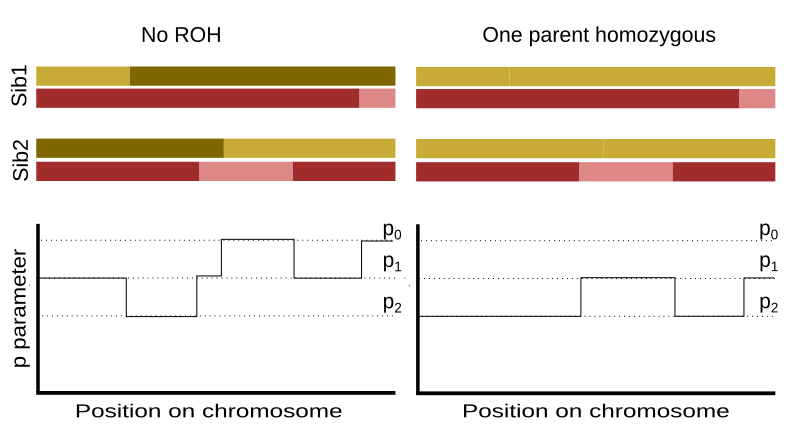
\includegraphics[width=18cm]{plots/inkscape_finalImg/schematic_sib.png}
    \centering
    \caption{IBD sharing between siblings with and without ROH. In top row, recombined chromosomes inherited from parents by a pair of siblings are shown. On left, the parents have unrelated chromosomes, and on right one parent has homozygous pair of chromosomes. Bottom row shows the expected proportion of differences along the chromosome in both the cases.}
    \label{fig0:schematic}
\end{figure}


There are numerous methods that utilize population allele frequencies, phase information, recombination maps, or genotype calls to estimate the relatedness coefficient \cite{huff_maximum-likelihood_2011,li_relationship_2014,li_accurate_2014,thornton_estimating_2012}. PLINK, a popular tool to infer relatedness coefficient in  diploid genotype data, estimates IBD probabilities from average of observed IBS, and using the allele frequencies at each SNP in samples \cite{purcell_plink_2007}. KING is another widely used software that allows relatedness inference with genotype data in homogeneous populations using population allele frequencies (KING homo), but can also work with structured populations with no good population allele frequencies using heterozygosity estimates from each sample (KING robust) \cite{manichaikul_robust_2010}. . 

\begin{table}
\caption{\label{tab:Table 1}IBD sharing probabilities for different relations}
\begin{tabular}{|c|c|c|c|}
    \hline
    Relatedness & $k_0$ & $k_1$ & $k_2$\\
    \hline
    Unrelated & 1 & 0 & 0\\
    \hline
    3rd Degree & 0.75 & 0.25 & 0\\
    \hline
    2nd Degree & 0.5 & 0.5 & 0\\
    \hline
    Siblings & 0.25 & 0.5 & 0.25\\
    \hline
    Parent-Child & 0 & 1 & 0\\
    \hline
    Identical/twins & 0 & 0 & 1\\
    \hline
\end{tabular}
\label{table1}
\end{table}

\subsection{Problems with ancient data, and methods that address these issues}
One major issue with applying above mentioned methods to ancient DNA is that, frequently, the amount of endogenous DNA is very low, making it very difficult to get genotype calls.
Several methods solve this problem by using genotype likelihoods \cite{lipatov_maximum_2015,korneliussen_ngsrelate_2015}. These methods account for the uncertainity in genotype calls by summing over all possible genotypes, weighted by the genotype likelihoods. However, these approaches typically still require at least 2x coverage, since genotype likelihoods may not be very informative at lower coverages. Apart from the low amount of endogenous DNA sequences present, ancient DNA analyses often have additional problems like contamination from modern populations \cite{peyregne_authentict_2020}, absence of a good reference panel, and ascertainment bias in case of captured sequences. In cases where allele frequency or a reference panel for the target population is not available, it is possible to use allele frequency from a modern population from the same geographic location, or to try using population allele frequencies from multiple potentially close populations. However, incorrect assumptions may cause the individuals in the target population to look more similar or different to each other \cite{amorim_understanding_2018}. Several methods have been proposed to estimate relatedness without a reference panel, but many of these require either $>4x$ coverage to get a good estimate of genotype likelihoods\cite{waples_allele_2019}, or a large sample size to get an estimate of population allele frequencies from the samples \cite{theunert_joint_2017}. In this study, we show that contamination from modern humans can cause some of the individuals in ancient populations to look more unrelated than they are. This happens because of comparison of endogenous reads to contaminating reads which would give higher differences than comparison of endogenous reads from individuals from ancient population. Hence, contamination can reduce the power to detect related pairs, especially when the target population is quite diverged from contaminating population(s). In addition, the target populations may have long runs of homozygosity (ROH) due to a small population size, or recent inbreeding. Long ROH causes related individuals to seem genetically closer to each other, while does not affect the genetic distance between unrelated individuals. This effect may cause an increase in false positives. In many cases, ancient DNA is captured with a SNP array, and the SNPs are ascertained to variable sites determined from certain individuals. Relatedness methods based on the fraction of sites in different IBS states are highly sensitive to ascertainment bias. KING robust, for example, differentiates between different relatedness by plotting KING‐robust kinship against fraction of sites in IBS0 \cite{manichaikul_robust_2010}. Another method from Rosenberg,2006 \cite{rosenberg_standardized_2006} uses the fraction of sites in all three IBS states to classify related individuals in the HGDP-CEPH Human Genome Diversity Cell Line Pane. These methods may give different results when applied to data with different ascertainment schemes \cite{waples_allele_2019}. 

READ is a software that does not require population allele frequencies or a reference panel, and can work with around 0.5 x coverage in presence of ascertainment bias. The software addresses the problem of unavailability of genotype calls by randomly sampling alleles from each individual. A string of these alleles at each position (called pseudohaploids) are then compared to other individuals to calculate pairwise genetic distances, which in turn are used to infer relatedness. The limitations are that the software can identify upto only second degree relatives, without differentiating between siblings and parent-child, which may be crucial when making pedigrees. 

\subsection{How our method works}
Here, we present KIn (Kinship Inference), a Hidden Markov Model (HMM) to estimate relatedness from low-coverage ancient DNA data. KIn can detect up to \nth{3} degree relatives, and differentiates between siblings and parent-child. KIn is also able to incorporate ROH, contamination and ascertainment bias. We validate the performance of KIn using simulations and show that we are able to infer relatedness in a neandertal data set, and a Bronze age dataset.



\section{Methods}

The core of  KIn, is a HMM that aims to infer relatedness and IBD sharing between a pair of low-coverage individuals, optionally taking ROH tracts in each sample, and contamination estimates into account. If the locations of ROH tracts are unknown, we provide another HMM to estimate ROH in the first step for a sample of sufficient coverage ($\geq 0.5x$). In a second step, the relatedness-HMM uses the contamination-corrected differences between a pair of individuals, and the positions of ROH tracts, to infer relatedness. Our method is available on \url{https://github.com/DivyaratanPopli/KIn_snakemake} along with a \textt{snakemake} \cite{koster_snakemakescalable_2012} pipeline to generate the input files for the models directly from bam files. 


\subsection{Relatedness Model overview} 
To estimate the relatedness of two individuals, we subdivide the genome into $L$ large windows $w$ (typically of size 10Mb). The inputs of our algorithm are i) the number of sites $N_w$ for which both samples have at least one read available, ii) the number of pairwise differences $D_w$ at these sites, and iii) probability of ROH in in windows, by default obtained from ROH-HMM described in a following section. Calculation of $N_w$ and $D_w$ requires comparison of reads at all positions for a pair of individuals. For low coverage genomes, this can be done by comparing randomly sampled read at each position for a pair of individuals (or by comparing pseudo haploid sequences). However, we realized that such random sampling can throw away a lot of useful data. To avoid this wastage, our input generation pipeline for Relatedness HMM calculates proportion of reads with alternate allele, at all positions for each genome. We use these proportions to find pairwise heterozygosity as the probability of comparing different alleles. These probabilities are summed up in each window to give $D_w$, along with the number of overlapping sites $N_w$.

Throughout, we will use bold-face notation to refer to the vector (or matrix) collecting  all the terms, e.g. $\BD = (D_1, D_2, \dots D_L)$. 

The model then uses this data for a given pair of individuals to classify each window into three hidden states $Z_w \in$ ($i_0$, $i_1$, $i_2$), reflecting zero, one or two chromosomes shared IBD. Likewise, we classify each window into one of three possible ROH state $H_w \in$ ($\omega_0$, $\omega_1$, $\omega_2$), reflecting, neither, one or both individuals being in a run-of-homozygosity at this genomic location.

Ideally, we would like to compute the likelihood $P(\BD | \BZ, \BH, \theta)$, where $\theta$ is a vector of parameters (initial transition probability $\pi$, transition matrix $A$ and $N_w$). 

However, calculating this likelihood is hard because the number of possible states for $\mathbf{Z}$ is very large, and we use a standard trick for fitting HMMs, to base or inference on the complete data likelihood:


\begin{align}
P(\mathbf{D},\BZ, \BH|\theta) &= P(\mathbf{D}|\mathbf{Z},\BH, \theta) P(\BZ |\theta)P(\BH |\theta) \nonumber\\
&= \prod_w P(D_w|Z_w,H_w, \theta) \prod_w P(H_w |\theta) \prod_w P(Z_w |Z_{w-1},\theta) P(Z_0|\theta)
\label{eq:1}
\end{align}


Here, $P(D_w|Z_w,  H_w, \theta)$ is the emission probability for window $w$,  $P(Z_w|Z_{w-1},\theta)$ is the transition probability, and $P(Z_0| \theta)$ is the initial probability $\pi$. $P(H_w |\theta)$ is the output of ROH HMM described in a following section.

Using the complete data likelihood allows us to factor the emission and transition probabilities, and hence we can maximize them independently.
Transition matrix for different cases of relatedness are either derived from theory, or obtained from simulations (see section). Initial transition probability $\pi_i$ is same for all the $i$.

\subsection{Emission probability}
In equation \ref{eq:1} the term $P(D_w | Z_w, H_w, \theta) = P(D_w | Z_w, H_w, N_w)$ is the emission probability, i.e. the probability of our data , given a particular hidden state. The number of shared sites $N_w$ is the only parameter in $\theta$ that affects the emissions.

Assuming sites are equally distributed and independent, we could use a  binomial likelihood
$$P(D_w|Z_w, N_w, H_w) \sim \text{Binom}[D_w ;N_w, p(Z_w, H_w)] \text{,}$$

where, $p$  is the expected proportion of differences we would expect for a particular IBD and ROH state.

If the two individuals are unrelated in a particular window and neither is in a ROH region (i.e. $Z_w = i_0$, and $H_w = \omega_0$), then the expected proportion of pairwise differences depends solely on the effective population size, and we denote this proportion with $p_0$. If the two individuals share one or even both copies of the genome IBD, we would expect the proportion of differences to be reduced to $p_1 = \frac{3}{4} p_0$, and $p_2 = \frac{1}2 p_0$, respectively, since either one or two of the four possible comparisons will be between identical chromosomes.


$p_0$, $p_1$, and $p_2$ are the expected proportion of differences in $i_0$, $i_1$, and $i_2$. $p_0$ is calculated directly from the data by calculating median of differences for all possible pairs of specimens. We calculate $p_1$ as $(3/4)p_1$ and $p_2$ as $p_1/2$. However, we need one more parameter (represented as $p_3$ in the matrix below) in cases where IBD state is $i_1$ and ROH state is $\omega_2$, or IBD state is $i_2$ and ROH state is $\omega_1$ or $\omega_2$. In such cases the expected proportion of differences between the individuals should be 0. However, as mentioned before, we do all our calculations in large windows, and start/end positions of these windows may not coincide with that of ROH tracts. And so, the pairwise differences in this state (called $p_3$ in the table) can lie anywhere between 0 to $p_2$. We found $p_3$ = $p_2$/2 to be a reasonable assumption for expected pairwise proportion of differences in this IBD/ROH state.


Taken together, we can summarize $p$ as follows 
\begin{equation}\label{eq:2}
    p(Z_w, H_w) = \left[\begin{array}
{rrr}
p_0 & p_1 & p_2 \\
p_0 & p_2 & p_3 \\
p_0 & p_4 & p_3
\end{array}\right]
\end{equation}



The effect of these considerations is that even though we have nine possible combinations of $Z$ and $H$ for each window, there are actually only four different $p$-parameters $p_x$ with $x$ $\in$ (0,1,2,3).



However, we find that the data often has considerably higher variance than would be expected from a binomial distribution, likely because we average over a large number of SNPs with different allele frequencies. 

We therefore add an overdispersion parameter $\delta$ that allows for variation in the $p$ between SNPs. This results in the betabinomial likelihood, (we show that such a distribution fits the data well (fig. S\ref{FigS1:binom})).  

\begin{equation}\label{eq:3}
P(D_{w}|p_x,\delta_x,N_w) = \binom{N_w}{D_w}\frac{B(D_w+p_x \delta_{x}, N_w-D_w+ \delta_{x}(1-p_{x}))}{ B(p_{x}\delta_{x}, (1-p_{x})\delta_{x})}
\end{equation}


\subsubsection{Estimation}

Emission probabilities are estimated with Expectation-Maximization (EM) algorithm. In each iteration of the algorithm, the Expectation step involves forward-backward algorithm to calculate joint probability of the observed data and the IBD states $Z$, given an initial guess of $\delta$. In maximization step we use these joint probabilities to optimize $\delta$, and update emission probabilities. Iterations are run, until the complete data likelihood stops changing. 

\paragraph{Initialization}
The value of $\delta$ is unknown to start with, and is randomly assigned, such that the mean of beta distribution and variance is within constraints described in maximization section.

\paragraph{Expectation step}

In this step, using the standard forward-backward algorithm, we calculate the posterior probability of each IBD state in each window ($\gamma_{wi}$). Expectation step, among other parameters, requires emission probabilities. We calculate emission probabilities for each case of $Z_w$ and $H_w$ from $\delta$ and $p$ using equation \ref{eq:3}, and we get the total emission probabilities for each $Z_w$ as $\sum_{H_w} P(D_w|Z_w,N_w,H_w) P(H_w|\theta)$

\paragraph{Maximization step}

The only free parameters we estimate in the M-step are the overdispersion parameters $\delta_j$. We do this optimization using a cost function, which is the log-emission probability weighted by the posterior probabilities of the hidden states $\gamma_{wi}$ and the ROH state-probabilities $h_{w\omega}$.


\begin{equation}\label{eq:4}
\mathcal{C} = \sum_{w=1}^L \sum_{i=0}^2\sum^2_{\omega=0} \log P(D_{w}|Z_w, H_w, N_w, \delta, p)h_{w\omega}\gamma_{wi}
\end{equation}


Using equation \ref{eq:2}, we simplify this by grouping all the terms that would result in the same $p$, i.e.

\begin{align*}
k_{w0} &= \gamma_{w0}\\
k_{w1} &= \gamma_{w1} h_{w0}\\
k_{w2} &= \gamma_{w2} h_{w0} + \gamma_{w1} h_{w1}\\
k_{w3} &= \gamma_{w2} h_{w1} + \gamma_{w2} h_{w2} + \gamma_{w1} h_{w2}
\end{align*}

So we can rewrite equation \ref{eq:4} as:
\begin{align}
\mathcal{C} &= \sum_{w=1}^L\sum_{x=0}^3 \log P(D_{w}|Z_w, H_w, N_w, \delta_x, p_x)k_{wx}
\end{align}

Since each term in this equation depends on only one $\delta_x$, we can optimize for them independently. For convenience, we refer to these four states corresponding to different $p$ as $x$ states.


We observed that estimating the $\delta_w$ without constraints can result in wide Beta distributions with very high variance, leading to over fitting of data (fig. \ref{figS4:bndsbeta}), and resulting in incorrect posterior probabilities for $Z_w$ (fig. \ref{figS3:bnds}). For example, a parent shares exactly one chromosome IBD with its child throughout the genome, so we expect only one IBD state. However, running an unconstrained model could use this data to fit a pair of siblings with a very wide beta-distribution (with a very high $\delta_1$, which may result in problems in differentiating between parent-child and siblings.

We avoid this problem by constraining the parameter space of $\delta$. 
In particular, 
Variance of beta distribution is shown below:
\begin{align}
    X \sim B(p,\delta)\\
    var(X) = \frac{p(1-p)}{\delta + 1}
\end{align}
We find the value of $\delta$ for which the variance is less than a threshold t.

We solve the following equation for $\delta$:
\begin{equation}
    \frac{p(1-p)}{\delta + 1}  < t
\end{equation}

We choose t for each beta distribution to be proportional to the mean ($p$), since the variances of beta distribution corresponding to different $x$ states follow the same relation as the distribution means. 
\begin{align}
    Var(X_{x_1}) = 3/4 Var(X_{x_0})\\
    Var(X_{x_2}) = 1/2 Var(X_{x_0})
\end{align}

Even though this may not hold true when we bin sites in large windows, we still find that $Var(X_{x_0}) > Var(X_{x_1}) > Var(X_{x_2})$ (fig. \ref{FigS1:binom}).

Ideally, t for $x_4$ should be zero, but since our genomic windows may not coincide with the IBD fragments or ROH, the variance can be much higher. We find that fixing t for $x_4$ at the same value as $x_0$ works well.



\subsection{Relatedness classes}
This model is run for different cases of relatedness including (Unrelated, $5^{th}$ Degree, $4^{th}$ Degree, $3^{rd}$ Degree, Grandparent-Grandchild, Avuncular, Half-siblings, Parent-Child, Siblings, Identical) using the corresponding transition matrix, and the likelihood for all the relatedness models is compared. We realized that we have low power to detect $4^{th}$ and $5^{th}$ degree and we can not always differentiate these from unrelated. In our final output, we show classifications of $4^{th}$ and $5^{th}$ degrees as unrelated. Similarly, we observe that we have low power to differentiate between half-siblings, avuncular and grandparent-grandchild, and we merge these classifications as $2^{nd}$ Degree in the final results. The relatedness for the maximum likelihood model is reported, and the confidence is given by the log likelihood ratio between the two highest likelihood models.  
Hidden IBD state of each window ($Z_w$) is estimated using standard Viterbi algorithm, and $\BZ$ corresponding to the most likely model are returned. 


\subsection{ROH estimation model}

Our HMM to detect ROH tracts works similar to the relatedness model described above. We sample all possible pairs of reads from each individual at all the positions where there are at least two reads, and calculate the proportion of read pairs that are different. These proportion of differences at each position are summed up in windows along the genome. This forms the input to the HMM, along with the number of overlapping sites, and the output is the posterior probability of a window being homozygous. This probability can also be inferred as the proportion of a window that has ROH. Our model has two hidden states: homozygous ($y_0$), and non homozygous ($y_1$). $Y_w$ denotes the state $y$ in a window $w$, and the vector of $Y_w$'s is denoted with $\mathbf{Y}$. The complete data likelihood for the model in this case is shown below:

\begin{align}
    P(\mathbf{\Delta},\mathbf{Y}|\Theta) &= P(\mathbf{\Delta}|\mathbf{Y},\Theta) P(\mathbf{Y}|\Theta)\nonumber\\
 &= [\prod_{w} P(\Delta_w|Y_w, \Theta) \prod_{w} P(Y_w|Y_w-1, \Theta)] P(Y_0| \Theta)
\end{align}


In this case, transitions are not known, and both transitions and emissions are estimated with standard EM algorithm. The emissions are calculated using betabinomial likelihood, and the mean of the distributions are constrained at expected proportion of differences in a ROH tract ($\rho_{0}$) and expected proportion of differences in a non-ROH tract $\rho_{1}$. Parameters $\rho_{1}$ and $\rho_{0}$ are the same as $p_{2}$ and $p_3$ in previous model. 

\subsection{Emissions}
Similar to our relatedness model, we estimate emissions using EM algorithm with expectation and maximization steps. The expectation step outputs the posterior probability $\Gamma$ of being in $y_0$ and $y_1$ in each window. Maximization step uses the $\Gamma$ to optimize overdispersion parameter $\eta$ with a betabinomial cost function:

\begin{align}
\mathcal{C} = \sum_{w} \sum_{y} P(\Delta_w|\eta_{wy},\rho_{wy}) \Gamma_{wy} 
\end{align}

In case of very noisy data, we see high pairwise differences in some windows that are not explained with the betabinomial distributions estimated for $y_0$ and $y_1$. To avoid our distributions from flattening to explain these high differences, we force these high difference windows to $y_1$ (fig. S\ref{figS5:ROHforced}). 

\subsection{Transitions}
Transitions are estimated using standard Baum-Welch algorithm. Expectation step is the same as that for emissions, and gives the posterior probability. In maximization step, we use the posterior probability to count how many times transitions are made from state i to j, normalized by the total number of times we are in state i. We observe that the final results are not affected by initial guess of the transition probabilities and assign a probability of 0.8 to stay in the same state for both $y_0$ and $y_1$. 

\subsection{Contamination}

Contamination by present-day people is a common feature in ancient DNA \cite{peyregne_present-day_2020} . Even low levels of contamination may make samples look less similar, and thus distort relatedness analyses. This issue is particularly pronounced  when analyzing populations with  low diversity, where even $<5\%$ contamination can cause loss of power to detect family relations. To address this issue, we  adjust $D_w$ and $N_w$, given the contamination estimates of both samples and the average divergence between the target population and a putative contaminating population.

For each pair of individuals $i$ and $j$ we approximate the contamination $C_{i,j}$ as the sum of contamination for each individual $C_i + C_j$. Then, $C_{i,j}$ represents the probability of comparing a contaminant read from an individual to an endogenous read from the other individual. Throughout, we assume that contamination levels are low, so that we can ignore comparison between contaminant reads, i.e. $C_iC_j \approx 0$.  We denote the average divergence between target and contaminating populations as $p_c$, and the observed proportion of differences between individuals $i$ and $j$ as $p_{oij}$. We calculate average endogenous pairwise difference $p_{eij}$ for individuals i and j as follows \cite{noauthor_ancient_nodate}:
\begin{align}
    p_{oij} = C_{ij}  p_c + (1-C_{ij})  p_{eij}\\
    or, p_{eij} = \frac{p_{oij} - C_{ij}  p_c}{1-C_{ij}} 
\end{align}

Given $p_{eij}$, we would ideally like to calculate the complete data log likelihood for the relatedness model while summing over all possible differences we could have in a window weighted by the probability of seeing that difference. 



\paragraph{Short version}
With contamination, we do not observe the number of differences $D_{true}$ and total number of comparisons $N_{true}$ directly, but instead need to approximate them. The window-subscript is omitted in the following for clarity:
\begin{equation}
    P(D_{\text{obs}} | N_\text{obs}, Z, \theta) \approx 
    P( \hat{D} | \hat{N}, Z, \theta)
\end{equation}
We do that by calculating the probability that a single read is endogenous given it has a difference.
\begin{align}
    \hat{D} = \mathbb{E}[D | D_{\text{obs}}, c] &= 
    D_{\text{obs}} P(E_i | D_i=1) \\
    &= D_\text{obs} \frac{P(D_i=1 | E_i)P(E_i)}{P(D_i=1)}\\
    &= D_\text{obs} \frac{(1-c)p_e}{(1-c)p_e + c p_c}
\end{align}

and likewise for reads that do not have a difference
\begin{align}
    \hat{S} = \mathbb{E}[S | S_{\text{obs}}, c] &= 
     S_\text{obs} \frac{(1-c)(1-p_e)}{(1-c)(1-p_e) + c (1-p_c)}
\end{align}

and $\hat{N} = \hat{S} + \hat{D}$

\begin{equation}
    P(D_{\text{obs}} | Z, N_\text{obs}, \theta) = \sum_n\sum_d P(D_{\text{obs}}, N_\text{obs} | D_w=d, N_w, C_i, C_j)\underbrace{P(D_w=d | N_w, Z, \theta)}_\text{old likelihood}
\end{equation}

i.e. we sum over all possible $D_w$, $N_w$. Instead, we use

\begin{align}
    P(D_{cor},Z|D,H,\theta,c,p_c) &= P(D_{cor}|Z,D,H,\theta,c,p_c) P(Z|D,H,\theta,c,p_c)\nonumber\\
    &= [\prod_{w} [\sum_\kappa P(D_{cor,w}|Z_w, H_w, \theta,c,p_c) P(D_{cor,w}=\kappa)] \prod_{w} P(Z_w|Z_{w-1}, \theta)] P(Z_0| \theta)
\end{align}



We realize that this calculation would be time consuming, and would further complicate the HMM. To avoid this, instead of using weighted sum of all possible $\kappa$, we use $E(D_{cor,w}|Z_w, H_w, \theta,c,p_c)$. This simplifies the equation 21 to :

\begin{align}
    P(D_{cor},Z|D,H,\theta,c,p_c) &= P(D_{cor}|Z,D,H,\theta,c,p_c) P(Z|D,H,\theta,c,p_c)\nonumber\\
    &= [\prod_{w} P(E(D_{cor,w})|Z_w, H_w, \theta,c,p_c) \prod_{w} P(Z_w|Z_{w-1}, \theta)] P(Z_0| \theta)
\end{align}

We calculate $E(D_{cor,w})$ as shown:

\begin{align}
    E[N_e] + E[N_c] = N\\
    E[D_e] + E[D_c] = D
\end{align}

Probability of comparing endogenous reads at a site where we see a difference:
$$P(\xi | N = 1,D = 1)=\frac{(1-c) p_e}{c p_c + (1-c) p_e} $$
Probability of comparing endogenous reads at a site where we see no difference:
$$P(\xi | N = 1,D = 0)=\frac{(1-c)(1-p_e)}{c (1-p_c) + (1-c) (1-p_e)} $$
Expectation of number of endogenous comparisons in a window:
\begin{align}
    E[\xi | N, D] = D E[\xi | N=1, D=1] + (N-D) E[\xi | N=1, D=0]\\
    = D P(\xi | N=1, D=1) + (N-D) P(\xi | N=1, D=0)
\end{align}



Total number of endogenous sites showing a difference in a window: 
$$D_{cor,w} = D_w* \frac{p_e(1-c)}{p_e(1-c) + c p_c} $$
Total number of endogenous sites showing 0 difference in a window: 
$$S_{cor,w} = S_w* \frac{(1-p_e)(1-c)}{(1-p_e)(1-c) + c (1-p_c)} $$
Total number of endogenous sites in a window:
$$N_{cor,w} = D_{cor,w} + S_{cor,w}$$

This model outputs the contamination corrected number of differences and overlapping sites in each window.

\subsection{Simulations}

We use simulations both for estimating the transition matrices for all our models, and for testing and validating our algorithm. All simulations are performed using \textt{msprime} \cite{kelleher_efficient_2016}, followed by simulations of related individuals using a predetermined pedigree (Figure S1).

\paragraph{ Simulations for estimation of transition matrix}

For our simulations of background diversity, we simulated a haploid population (Pop1) with constant effective size of 10,000 and sampled 16 haploids from 2500 generations ago to randomly combine into 8 unrelated diploid ancient individuals (fig. \ref{figS10:pedigree}). For each individual, we simulated 22 chromosomes with length $L=100$ Mb. The mutation rate was set as $\mu= 10^{-8}$ per base pair per generation and recombination rate used was $r=10^{-8}$ 

For artificially mating two individuals, we simulated a recombined chromosome from each individual to be passed on to the progeny. For simulating a recombined chromosome from a diploid individual, we drew the number of recombination points from a Poisson distribution with parameter $rL$ as the recombination rate, and used a uniform distribution to sample the positions of recombination points. We estimated transition matrices corresponding to different cases of relatedness by counting transition between IBD states for a pair of  individuals at a particular relatedness level. We compared the transition matrices for grandparent-grandchild and siblings estimated in this way to a theoretical calculation, and verified that they are very close. However, it is difficult to theoretically calculate transition matrices for other cases like third degree, and so for these cases we use the transition matrices obtained from simulations.

\paragraph{Model Comparison}
Model with maximum likelihood is reported, and log likelihood ratio is calculated with the two highest likelihood models. 

Apart from the related and unrelated individuals in pop1, we simulated more haploids in three other populations to create scenarios with ascertainment and contamination (fig. \ref{figS10:pedigree}). We simulated two haploids to form an individual each from two other populations (pop2, pop3) with split time of 3500 and 4500 generations with pop1, and sampling time of 4000 generations and 2000 generations ago respectively. We identified the sites that were polymorphic among these two individuals, and used these sites to ascertain the genomes of individuals from pop1. We test out the performance of our method in presence of long ROH ($\sim17\%$), by simulating regions of homozygosity with a markov chain using transition matrix shown below: 

$$\mathbf{A} = \left[\begin{array}
{rr}
1-10/l & 10/l \\
2/l & 1-2/l  \\
\end{array}\right]
$$

Here, l is length of the chromosome. From the steps described above, we got genotypes of 17 individuals in pop1 in presence/absence of ROH and ascertainment. We further simulated 10 haploids (5 diploid individuals) from pop4 with split time of 20,000 generations with pop1, sampled from the present time. We calculated the allele frequency for pop4 at each site, and used it to introduce contamination (with fixed contamination percentage for each individual ($<5\%$) in samples from pop1. We generated reads (derived/ancestral) for different genomic coverages ranging from 4x to 0.03x at each position for each individual. We specifically generated reads for four different cases: Ancestral-Endogenous, Ancestral-Contaminant, Derived-Endogenous, Derived-Contaminant. The number of reads for each case was sampled from a Poisson distribution with $\lambda$ calculated from the coverage $\zeta$, allele frequency or genotype (G $\in$ 0,0.5,1), and contamination estimate:

\begin{align}
    \lambda_{DE} = \zeta (1-c) G\nonumber\\
    \lambda_{AE} = \zeta (1-c) (1-G)\nonumber\\
    \lambda_{DC} = \zeta c \upsilon\nonumber\\
    \lambda_{AC} = \zeta c (1-\upsilon)
\end{align}

\section{Results}

We predict the following categories of relatedness with KIn: Identical individuals (twins), First degree (parent-child), First degree (siblings), Second degree, Third degree, Unrelated (including higher than third degree relatives). We show the working of Relatedness HMM with Fig.\ref{fig1:ibd} showing performance of each model, when applied to a pair of siblings. 

\begin{figure}[h!]
    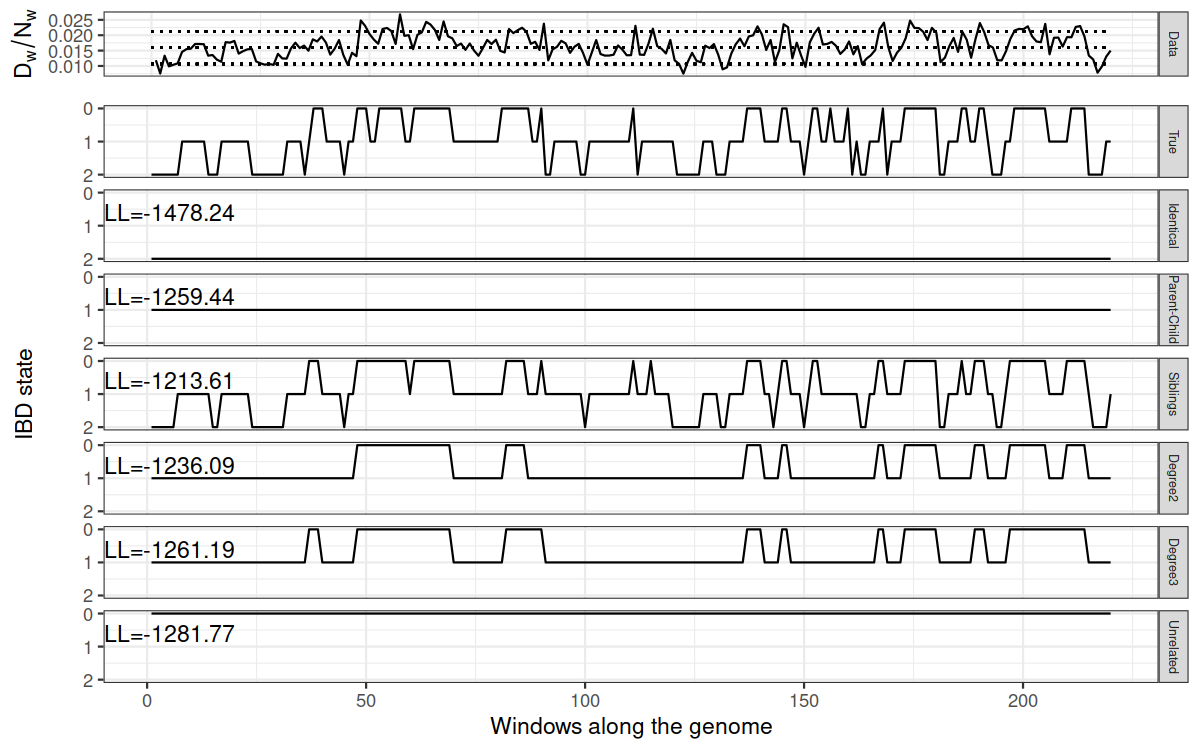
\includegraphics[width=16cm]{plots/plotimg/IBDplot.png}
    \centering
    \caption{Comparison of IBD fragments predicted by different relatedness models. Top panel shows the proportion of differences in each window along the genome for a pair of simulated siblings. Dashed lines in this panel represent $p_0$, $p_1$ and $p_2$ estimates. The panel just below shows the true IBD state for each window. Each panel below shows the IBD states predicted by a particular relatedness model. The log likelihood value for each model is shown on upper left corner of the panel. }
    \label{fig1:ibd}
\end{figure}


We see that in this case, the siblings model predictions match true IBD states the most. This is reflected in the log likelihoods values (LL) of the models as well, where siblings model has the highest value. We take a loglikelihood ratio ($\Lambda$) of the two most likely models to get a confidence in the relatedness estimate (in this case $\Lambda$ = 22.48). All the models in Fig.\ref{fig1:ibd} utilize information about ROH given by the ROH-HMM. 


Performance of ROH-HMM under different cases of ascertainment, contamination and long ROH, and for different coverages is shown in Fig.\ref{fig2:ROH}. We observe that as coverage decreases, data becomes more noisy. This causes ROH HMM to predict some probability of ROH in few windows when there is no ROH in data. However, at 4x and 0.5x, this is very rare. In presence of ROH, we see a similar trend. At 4x the model can estimate ROH probability well, but loses accuracy at 0.2x. In presence of ascertainment, overlapping sites are reduced, but they are informative. We see that the model performs well at 0.5x. New plot for contamination to be included. We applied the ROH-HMM and relatedness HMM on 60 runs of simulations, to get relatedness estimates, and compared the final relatedness estimates to the true relatedness for different pairs at coverages ranging from 4x to 0.1x. 

\begin{figure}[h!]
    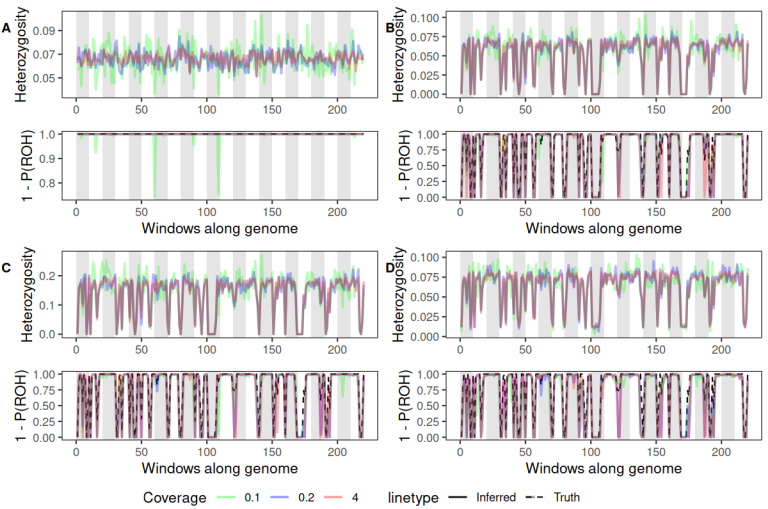
\includegraphics[width=16cm]{plots/inkscape_finalImg/ROHplot.png}
    \centering
    \caption{Estimation of ROH probabilities along the genome in simulations with different cases of ROH, contamination, and ascertainment. Top panel shows proportion of differences in a simulated individual along the genome, and the bottom panel shows probability of seeing no ROH. (A) Simulation with no ascertainment, contamination, or ROH. (B) Simulation with ROH. (C) Simulation with ROH and ascertainment. (D) Simulation with ROH and contamination.}
    \label{fig2:ROH}
\end{figure}


We plotted the true positive and false positive rates with a cutoff on the loglikelihood ratio in Fig.\ref{fig3:cutoff}. Here, and in Fig.\ref{fig4:Comparison_READ_KIn}, we have two relatedness labels: 'Unrelated' and 'Unrelated w/o 3rd Degree'. Unrelated label here refers to KIn performance results when all Unrelated, Fifth Degree, Fourth Degree, Third Degree pairs are labelled as Unrelated. This is useful for comparison to READ, since READ classifies relatedness upto Second Degree. 'Unrelated w/o $3^{rd}$ Degree' refers to the performance results when Third Degree is considered as separate from the unrelated individuals. Fig.\ref{fig3:cutoff} shows that for Identical, First Degree, Unrelated pairs, the false positive rate is below $5\%$ even when no cut off is used. For second degree, at 0.1x we see a high false positive rate, that does not go down much with an increase in cutoff. For the same relationship, at a coverage of 0.2x, a cutoff of 1 seems appropriate to reduce false positive rate to below $5\%$. Similarly, for siblings at 0.1x, a cutoff of 1 works well to keep false positives low. For parent-child, we find that a cutoff of about 2 is a better choice. Degree 3 shows higher false positive rates in general, and we see that only for 4x coverage and a cutoff of 2, do we see a false positive rate of around $5\%$. In conclusion, it is recommended to use a cutoff of 1 for most cases, with the exception of differentiation between parent-child and siblings, where a cutoff of 2 may be more appropriate, and degree 3 where cutoff of 2 at 4x coverage seems reasonable. 

\begin{figure}[h!]
    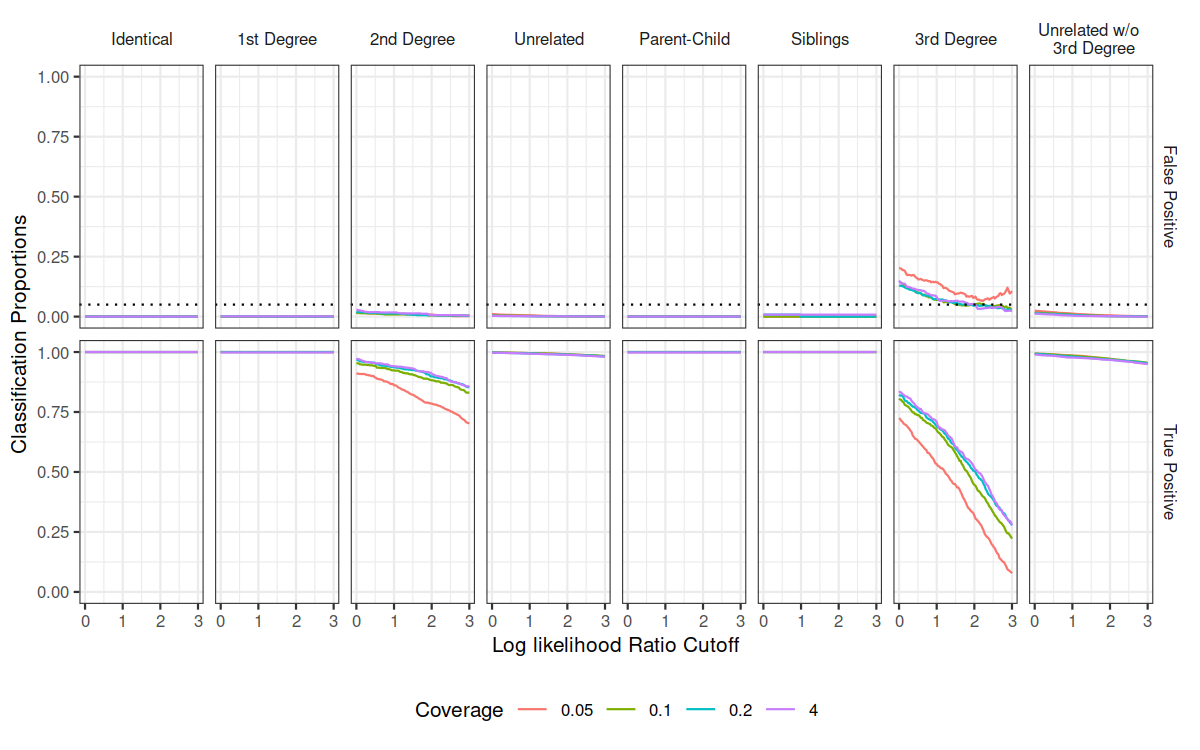
\includegraphics[width=16cm]{plots/plotimg/contam0_inbred0_model_performance_allroc_asc0_plot.png}
    \centering
    \caption{False positive and True Positive rates as a function of cutoff on log likelihood ratio. In top panel, dotted line represents $5\%$}.
    \label{fig3:cutoff}
\end{figure}

We use a cutoff of 1 to compare our method performance to READ, while using a cutoff of 1 standard deviation for READ. Fig.\ref{fig4:Comparison_READ_KIn} shows this comparison using false positive and true positive rates for both the methods at different coverages under different simulations. We show that both methods have similar performance in the control case (except for 0.1x coverage, where KIn has higher power to detect First Degree and Second Degree, and slightly higher false positive rate for degree 2). However, in case of ascertainment, ROH, or contamination KIn shows higher power to detect relatedness cases while maintaining a low false positive rate. 

\begin{figure}[h!]
    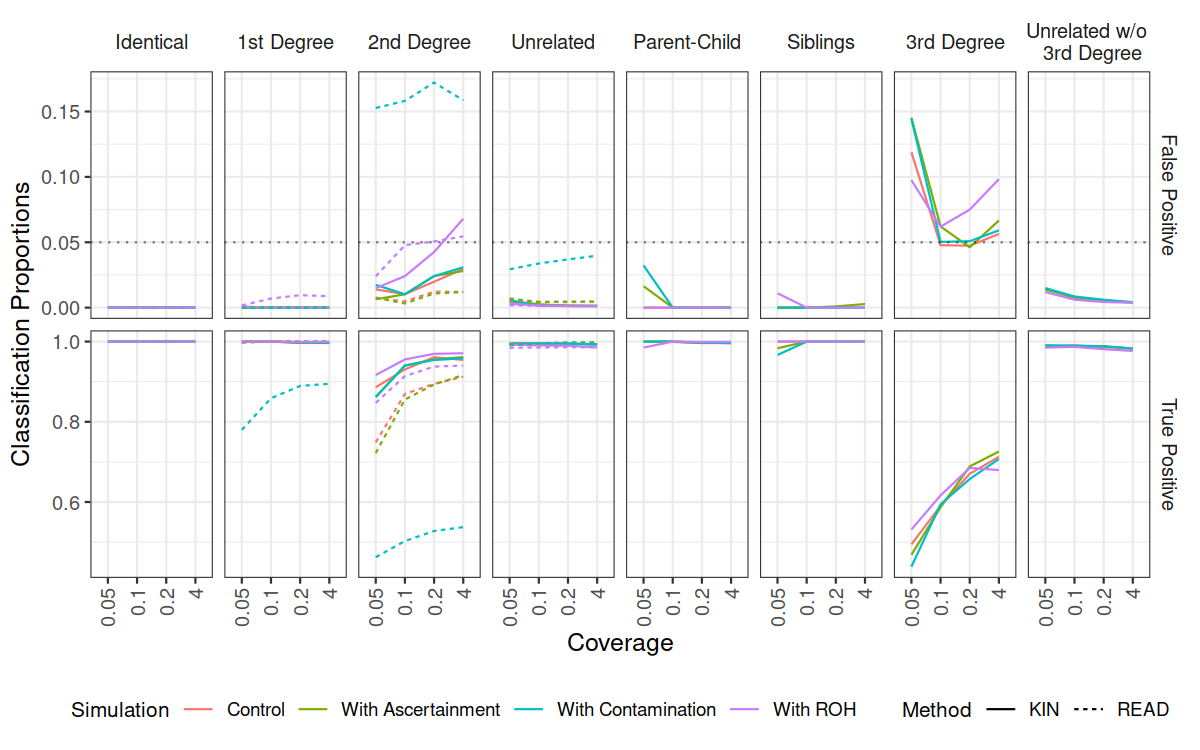
\includegraphics[width=16cm]{plots/plotimg/comparison_plot.png}
    \centering
    \caption{Comparison of KIn with READ using simulations with different coverages, and different cases of ascertainment, contamination and ROH}
    \label{fig4:Comparison_READ_KIn}
\end{figure}


To test KIn on real ancient dataset, we applied it to Neandertal specimens from Chagyrskaya cave in Siberia, Russia. This dataset comprised of 14 specimens that came from neighbouring layers, and hence could possibly belong to contemporary neandertals who occupied the cave 63 ± 4 to 48 ± 3 kya \cite{kolobova_archaeological_2020-1}. These specimens showed low coverage of nuclear genome, with 8 samples out of 14 showing $<1x$ coverage. Some of these specimens showed signs of long ROH, and contamination from modern humans as well as Hyena. All these samples were captured with an array targeting for Neanderthal variation, and we further ascertained this data to variable sites in high coverage Neanderthal genomes: Altai Neanderthal (Denisova 5) \cite{prufer_complete_2014} and Vindija 33.19 \cite{prufer_high-coverage_2017}. This dataset had all the issues that KIn deals with, and hence we decided to apply it here to see if we could find family relationships that would not be possible with other available methods. Our results for pairwise relatedness for these individuals is shown in Fig.\ref{fig5:Chagyrskaya_kin}. We found identical individuals (Chagyrskaya13-Chagyrskaya19-Chagyrskaya1141), first degree relatives (Chagyrskaya07-Chagyrskaya17, Chagyrskaya06-Chagyrskaya14), and a second degree relative (Chagyrskaya01-Chagyrskaya60). These results agree with READ (fig. S\ref{figS2:Chagyrskaya_READ}). Interestingly, for the pair of Chagyrskaya07-Chagyrskaya17, READ shows that they are first degree relatives, and KIn further identifies them as parent-child. Our result matches with the conclusions of the authors based on additional information from mtDNA. Further, we find a possible third degree relative (Chagyrskaya07-Chagyrskaya60). We compared our results to lcMLkin, and show that the software does not perform well with these low coverage samples since it is not possible to obtain reliable genotype likelihoods for many of these samples (fig. S\ref{figS6:Chagyrskaya_ibd}).



\begin{figure}[h!]
    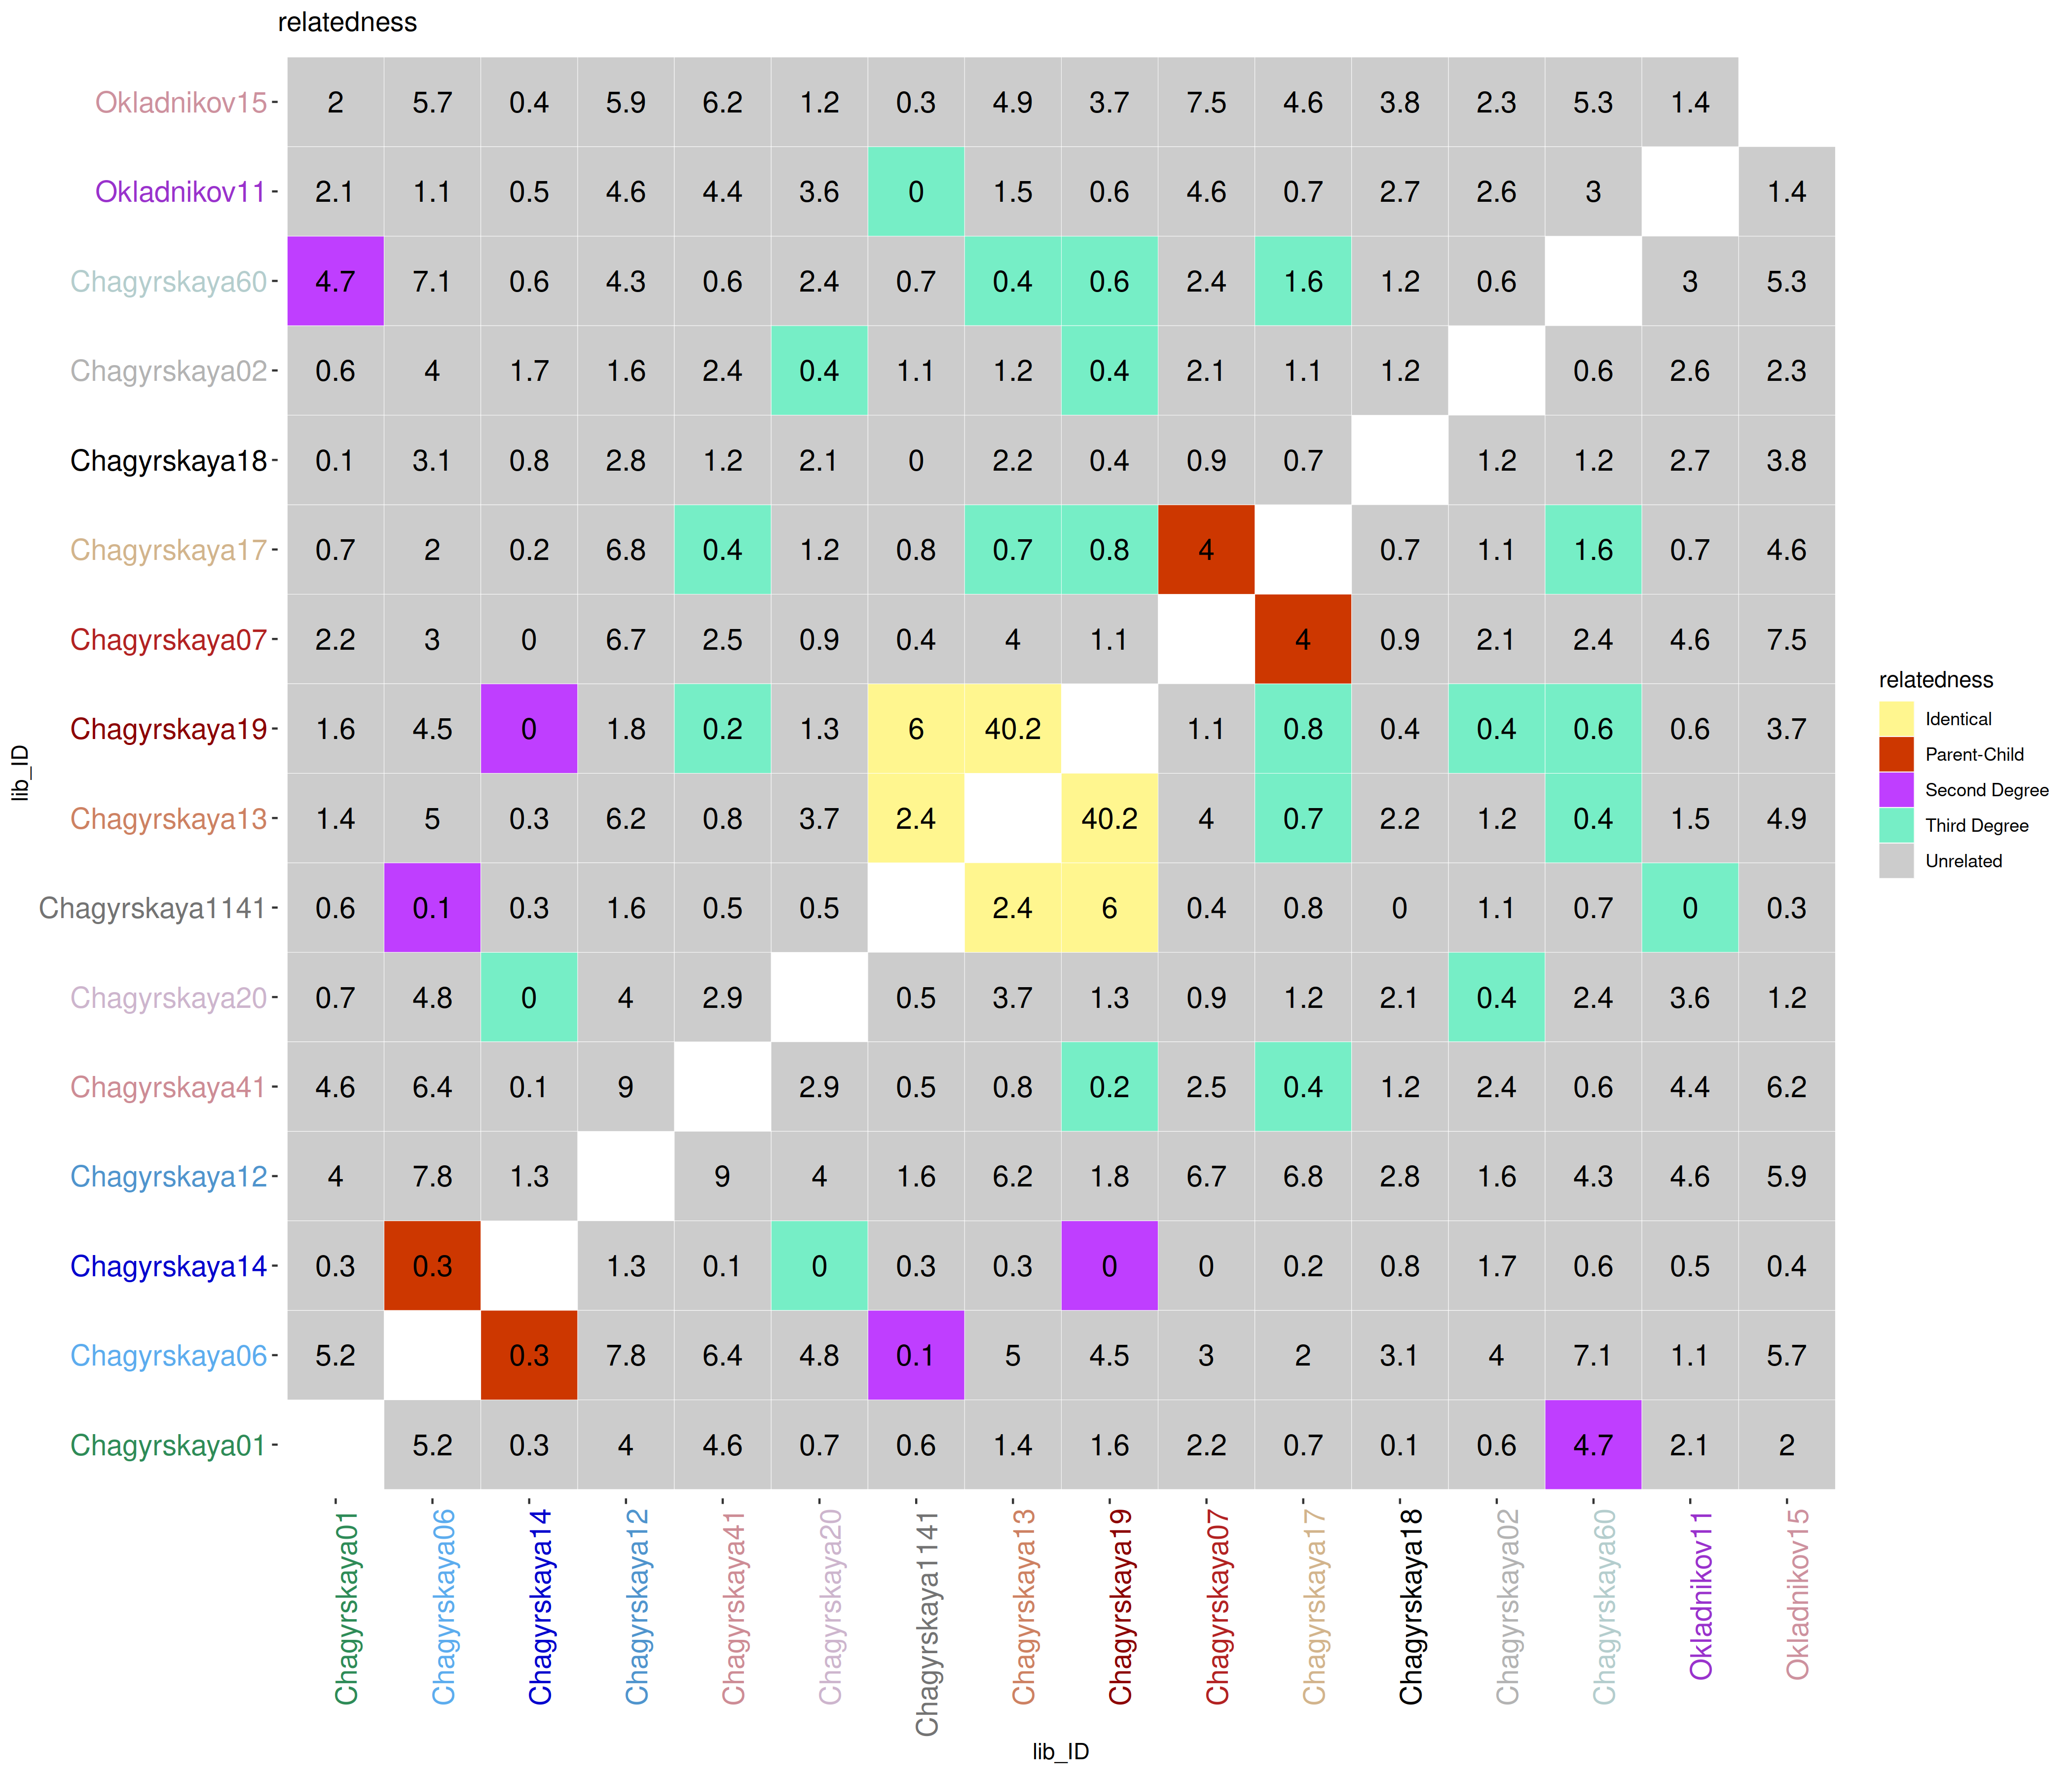
\includegraphics[width=18cm]{plots/plotimg/fil0_relatable_plot.png}
    \centering
    \caption{Application of KIn on Neandertal specimens from Chagyrskaya. Color of a square represents the relatedness, while the number denotes loglikelihood ratio between the two maximum likelihood models.}
    \label{fig5:Chagyrskaya_kin}
\end{figure}

We further applied KIn to a genome-wide dataset of 118 ancient individuals sequenced and analyzed by Mittnik et al.,2019. We compared our relatedness estimates to those obtained from the authors using READ and lcMLkin, and found that in most cases the three methods agree. Out of 6903 pairs, 346 pairs show different relatedness for KIn and READ (table S2). However, there are only 31 pairs where KIn has $log likelihood >1$. We looked in detail at some of these pairs, and we found that it is possible to deduct the correct relatedness for several of these pairs by plotting the proportion of differences along the genome. In all the pairs that we analyzed in this way, KIn seems to predict the true relatedness. We show few examples of such cases in fig. S\ref{figS8:eg1}. We found 20 pairs in this subset of 346 pairs where lcMLkin has sufficient data. Among these 20 pairs, we found that lcMLkin matches KIn estimate in all cases except for pair POST131-POST28 (READ predicts unrelated individuals, lcMLkin predicts 3rd-5th degree, KIn predicts second degree) and pair AITI72-AITI77A (READ and lcMLKin predict unrelated, while KIn estimates 3rd degree with log likelihood=1.7).  
We found 43 pairs for which READ estimates first degree, and compared the estimates of lcMLkin and KIn for these cases (suppl table3). There were a total of 20 pairs where lcMLkin had sufficient data, and 26 pairs where $loglikelihood ratio>2$ for KIn. Among the 19 overlapping pairs, we found four pairs where KIn and lcMLkin differ, and a visual inspection shows that in these cases, KIn seems to have the correct estimate (fig. S\ref{figS9:eg2}).  




\section{Discussion}

Several methods are available to estimate relatedness from modern as well as ancient DNA data. We develop a new method to estimate genetic kinship from low coverage data. We show that it is possible to accurately infer relatedness, along with IBD tracts, from such data in presence of long ROH, contamination, as well as ascertainment bias. Our method utilizes Hidden Markov Models to estimate IBD tracts, conditional on a particular relatedness, and we use log likelihoods of these HMMs to find the best fit. This approach of using Hidden Markov Model makes use of the fact that DNA is inherited in blocks, and hence the IBD state in a given window is dependent on the IBD state in the previous window. We use this approach to identify the following relatives: Identical individuals, Parent-Child, Siblings, Second degree, Third degree, Unrelated individuals. We show that it is possible to differentiate between avuncular and grand-parent-grandchild relations. We have developed a similar Hidden Markov Model to infer long ROH, and use the posterior probabilities to make better relatedness inference. We further use a simple model to correct the pairwise differences in genomic windows for contamination. 

We demonstrate using simulations, that our method performs well at low coverage. We compared KIn's model performance to a widely used software READ to show that our approach works at least as good as READ on ideal data without long ROH, ascertainment and contamination, while additionally distinguishing between parent-child and siblings, and identifying third degree relatives. We demonstrate that at low coverage (0.1x) we have higher power to detect first degree relatives compared to READ with similar false positives, while a higher power to identify second degree relatives at the cost of slightly higher false positive rate. Contrary to the intuition, we see that adding long ROH ($~17\%$) to simulations improves the performance of both KIn and READ. READ's performance improves because ROH does not cause any change in pairwise differences between unrelated individuals, while decreasing pairwise differences between related individuals. More is the relatedness, the more is the decrease in pairwise differences in presence of ROH. And so long ROH causes higher power for READ which otherwise is a conservative method. KIn performs well for the same reasons, but can miss-classify second degree individuals with ROH as siblings, if ROH is not accounted for. Hence, we implement ROH states in the relatedness model to avoid such miss classifications. Contamination, on the other hand can make the performance of READ much worse depending on the amount of contamination, and the number of individuals contaminated. We show that even at contamination levels  $<=3\%$, and contamination in only 8 out of 17 individuals, READ performance falls dramatically. Contamination in more individuals will cause a shift in median difference in the population and may cause non contaminated individuals to look more related, thus increasing the false positive rates. On the other hand, increase in amount of contamination in few individuals can make them look more unrelated. KIn, with the implementation of a model to account for contamination performs well in this case. Ascertainment causes a decrease in power for both the methods, since it reduces the amount of data. However, the decrease in power is more for READ compared to KIn.

DNA data from Bronze age, Lech valley has low contamination, and no ROH. We demonstrate that KIn matches the results from READ and lcMLkin for pairs with good amount of overlaps, while adds more information for low coverage samples. As expected from the simulations, KIn is helpful in differentiating between parent-child from siblings, and identifying second and third degree individuals in cases where there is an overlap of only few thousand sites or less, and the other methods are not informative. We show that when applied to neandertal specimens from Chagyrskaya cave, READ and KIn agree in relatedness estimates for all pairs where both methods have sufficient data. KIn additionally identifys a pair of first degree relatives as parent-child, which is also confirmed with mtDNA. In addition, KIn identifies a third degree relative. We compare IBD estimates from KIn to lcMLkin and show that KIn's IBD estimates are much closer to the expected estimates, given the relatedness between individuals that has been estimated with both READ and KIn. 
Output of KIn is a table which shows for each pair, the most likely model, and the second best guess, along with a confidence level represented by the log likelihood ratio. Due to the tabular output, KIn is easy to automatise and apply on large datasets. 
One limitation with our approach is that this method assumes a single population. In case of population structure, with the subpopulations with very different diversity, KIn may show inaccurate inferences. Our method makes another assumption, that the dataset comprises of at least some unrelated individuals. We estimate $p_0$ as the median of all pairwise differences, and if more than half of the pairs are related to each other, $p_0$ estimate would be biased, and may affect the relatedness inference. In this study, we identify six different cases of relatedness, but in theory our approach can be extended to identify many more such cases, such as double first cousins, using a corresponding IBD state transition matrix.


\section{Supplementary Information}

Pipeline of KIn

\renewcommand{\figurename}{Fig. S}
\begin{figure}[h!]
    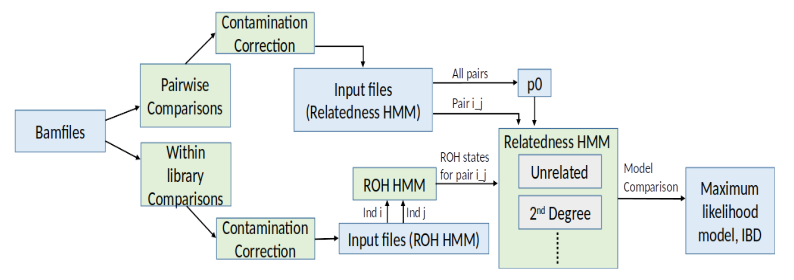
\includegraphics[width=18cm]{plots/inkscape_finalImg/schematic_sup.png}
    \centering
    \caption{Overall schematic of the method. Blue boxes show the data files, while green boxes represent scripts.}
    \label{figS0:schematic}
\end{figure}


Beta binomial distribution is a better fit compared to Binomial distribution for proportion of differences in windows.


\begin{figure}[h!]
    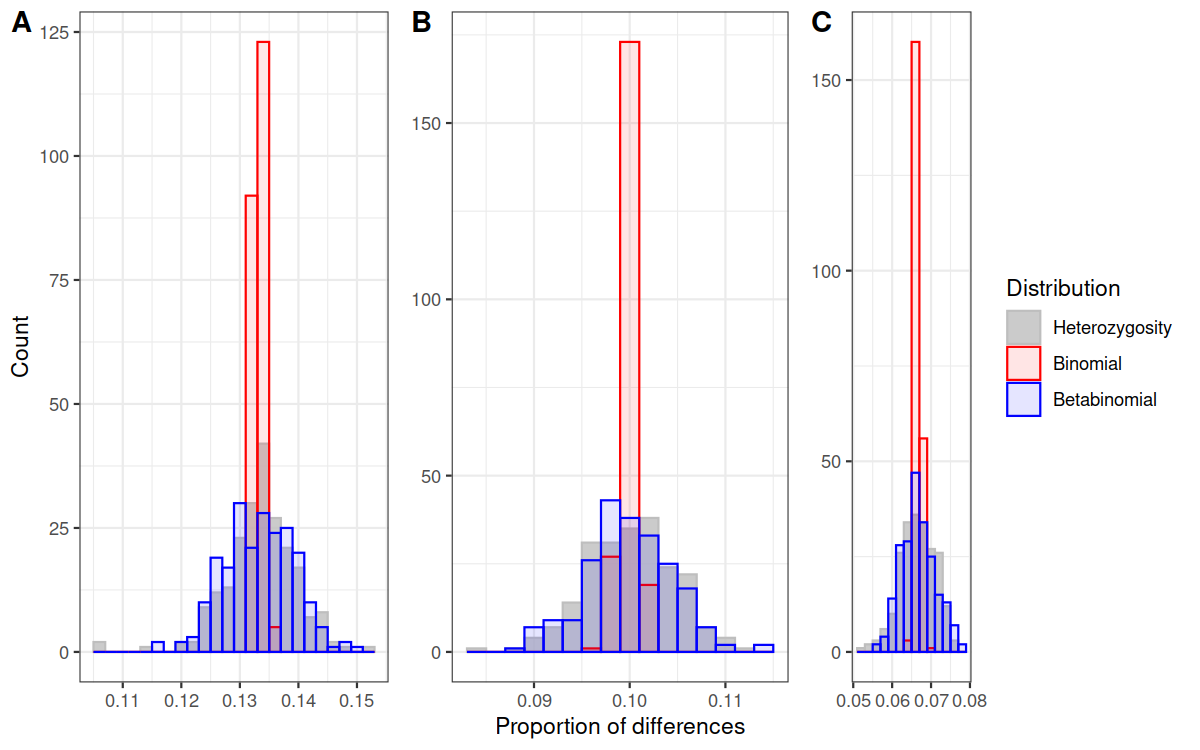
\includegraphics[width=18cm]{supplementary_info/plots/binom.png}
    \centering
    \caption{Comparison of fit with Betabinomial and Binomial distributions. Data is represented by the histogram of proportion of differences from all windows of a (A) unrelated, (B) Parent-Child, (C) Identical pair of individuals. Binomial parameter p is calculated from the data, while Betabinomial parameters are estimated with the relatedness HMM.}
    \label{figS1:binom}
    
\end{figure}


\begin{figure}[h!]
    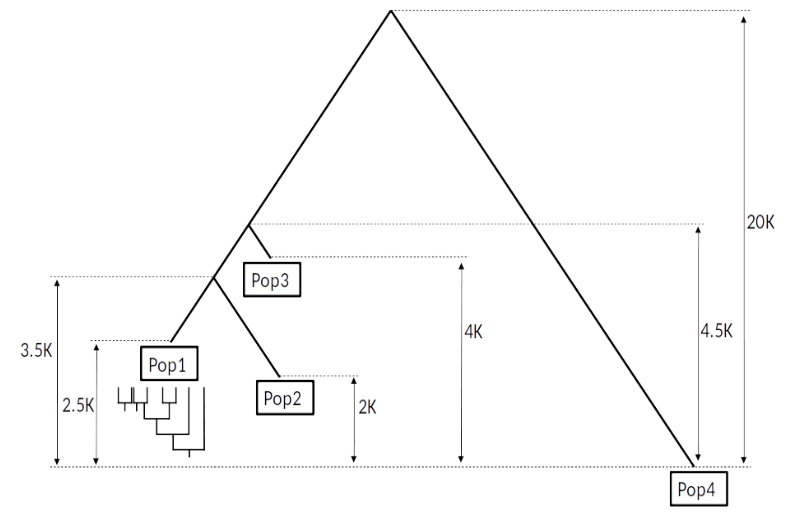
\includegraphics[width=18cm]{plots/inkscape_finalImg/pedigree.png}
    \centering
    \caption{Overview of simulated dataset. We simulate pop1, and artificially mate unrelated individuals to make a family with upto 5th degree relatives, along with other unrelated and identical individuals (not shown here). Pop2 and Pop3 are simulated so as to introduce ascertainment, while Pop4 is a present day population used to simulate contamination. Split times and age of the populations are shown in generations.}
    \label{figS10:pedigree}
    
\end{figure}


Results from KIn agree with results from READ, and provide some more information about siblings/parent-child, and $3^{rd}$ Degree relatedness. 
\begin{figure}[h!]
    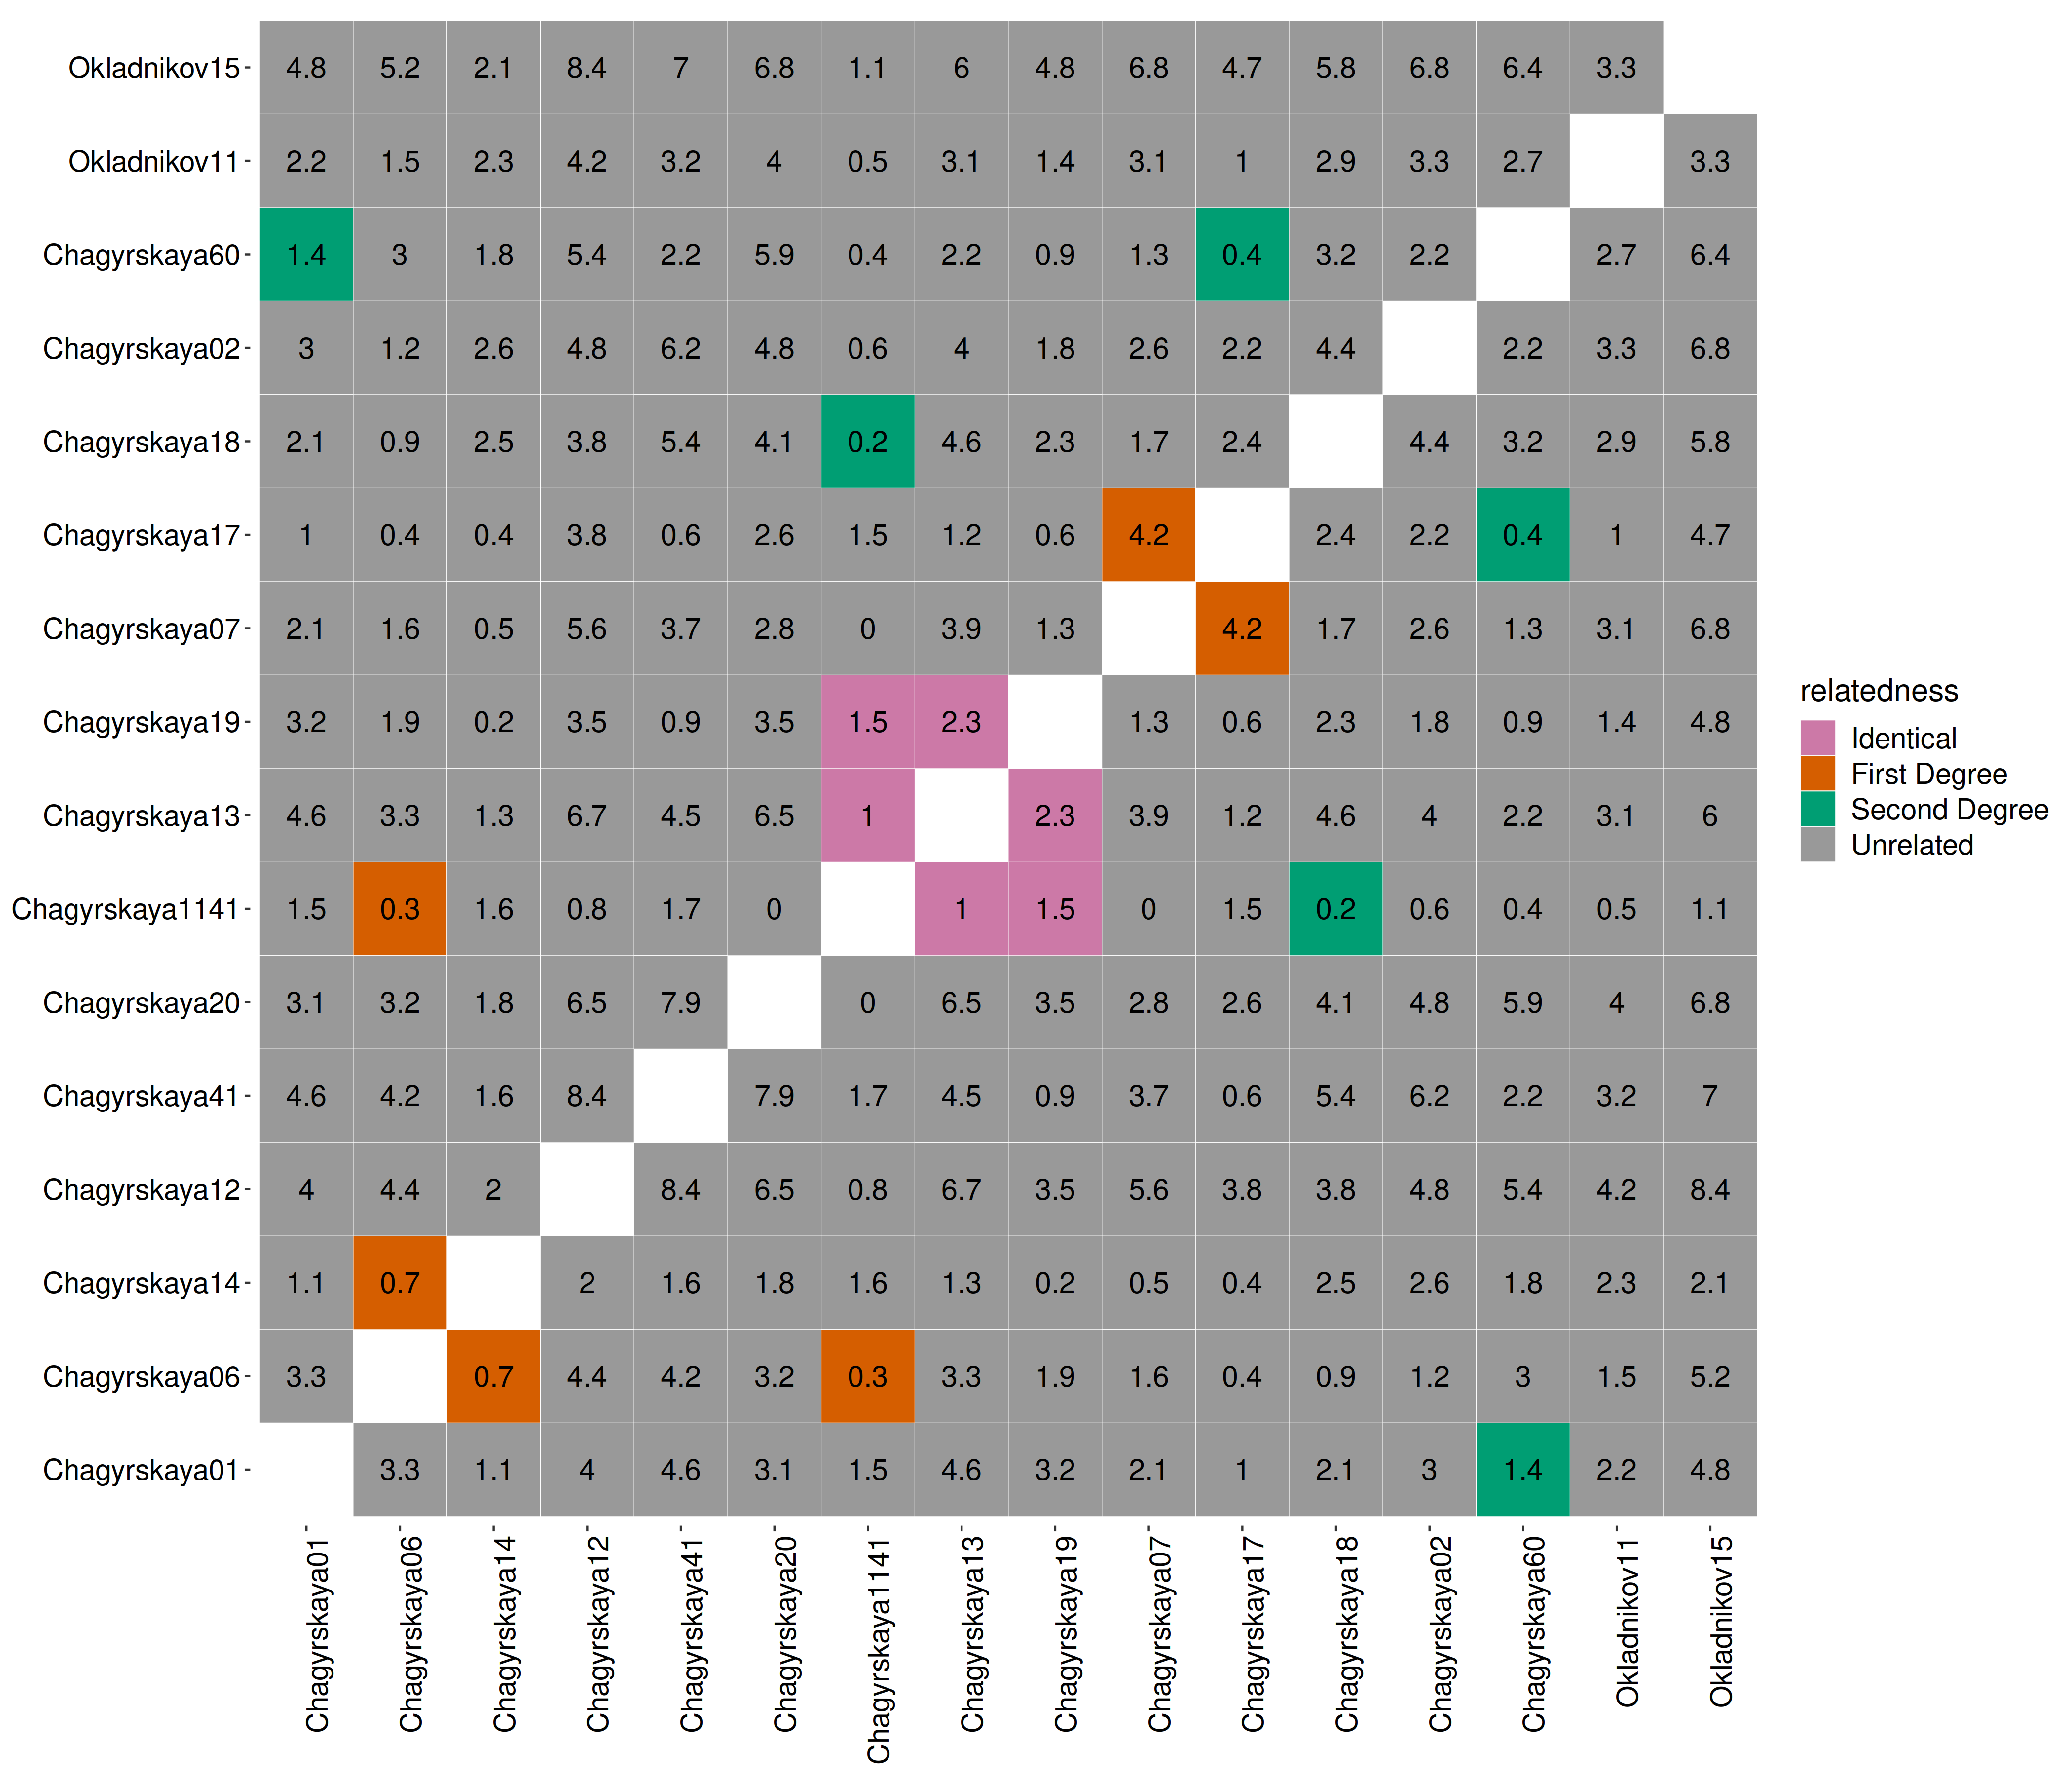
\includegraphics[width=18cm]{supplementary_info/plots/fil0_read_plot.png}
    \centering
    \caption{Application of READ on Neandertal specimens from Chagyrskaya cave. Color of a square represents the relatedness, while the number denotes standard deviations away from the upper threshold (we show lower threshold for unrelated pairs since upper threshold is not available).}
    \label{figS2:Chagyrskaya_READ}
\end{figure}

Constraining variance of beta distributions in case of an identical pair, when identical relatedness hmm is applied, gives more accurate emission probabilities.
\begin{figure}[h!]
    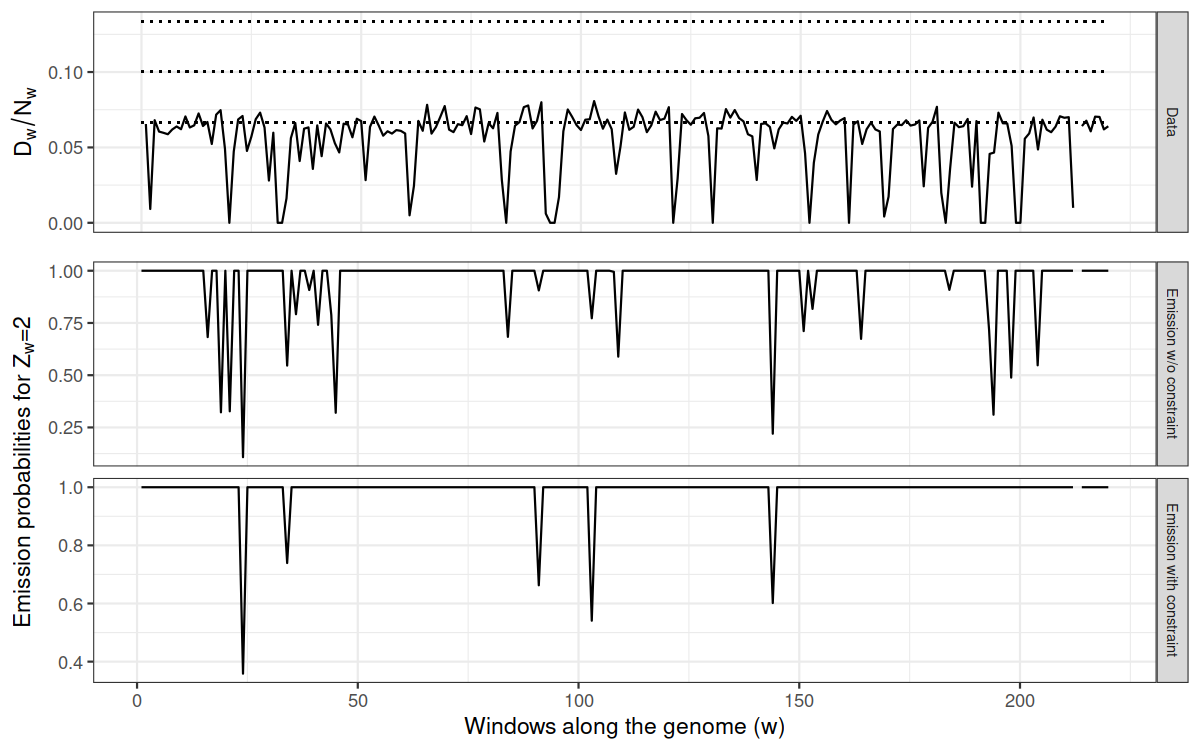
\includegraphics[width=18cm]{supplementary_info/plots/contam0_inbred1_run57_coverage0.2_asc0_inputMode_hapProbs_fil0_pair0_15_relid_emissions_bnds.png}
    \centering
    \caption{Application of identical relatedness HMM on a pair of identical individuals with low coverage (0.2x), and ROH tracts. Top panel shows pairwise proportion of differences is close to expectation, but dips in some windows due to presence of ROH tracts. Bottom two panels show $P(Data|Z=2)$ without constraints and with constraints respectively.}
    \label{figS3:bnds}
\end{figure}

In figS4, the emissions improve in accuracy with constraints on variance of Beta distributions. figS5 shows why we see this improvement. With variance constraints, beta distributions corresponding to Z=1 and Z=2 do not overfit the data, and higher emission probabilities seen in (A) at $D_w/N_w$=0.05 disappear. All probability distributions are scaled by the same factor so they are visible with the data histogram.
\begin{figure}[h!]
    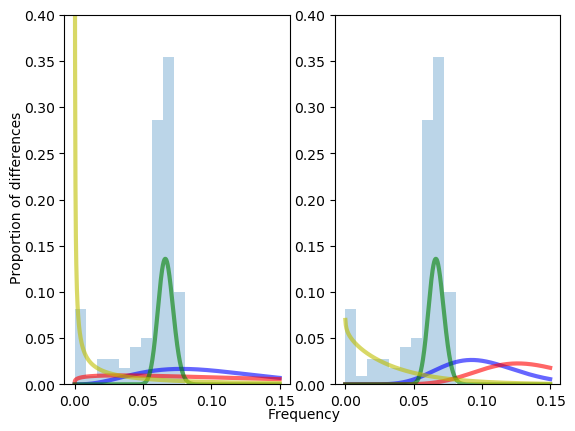
\includegraphics[width=18cm]{supplementary_info/plots/contam0_inbred1_run57_coverage0.2_asc0_inputMode_hapProbs_fil0_pair0_15_relid_betaplot.png}
    \centering
    \caption{Comparison of beta distributions estimated with the HMM (left) without and (right) with variance constraints.}
    \label{figS4:bndsbeta}
\end{figure}

Restricting the emission probabilities at 1 for Y=1, in windows that have higher than $p_0$ difference improves the estimated Beta parameters. 
\begin{figure}[h!]
    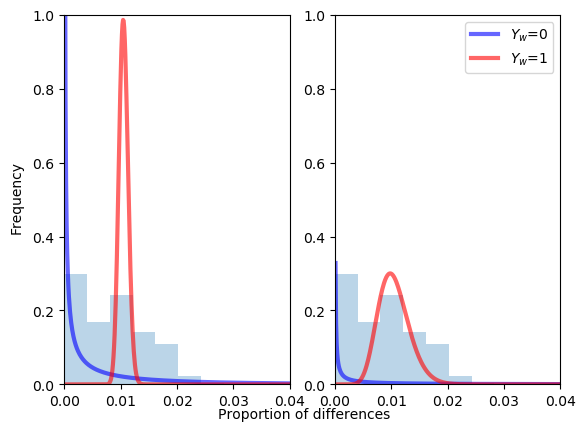
\includegraphics[width=18cm]{supplementary_info/plots/contam0_inbred1_run57_coverage0.2_asc0_inputMode_hapProbs_fil0_ind0_forced_roh.png}
     \centering
    \caption{Comparison of Beta distributions (left) without and (right) with modified emissions}
    \label{figS5:ROHforced}
\end{figure}

*Remember to use updated lcMLkin in the plot.
\begin{figure}[h!]
    \centering
    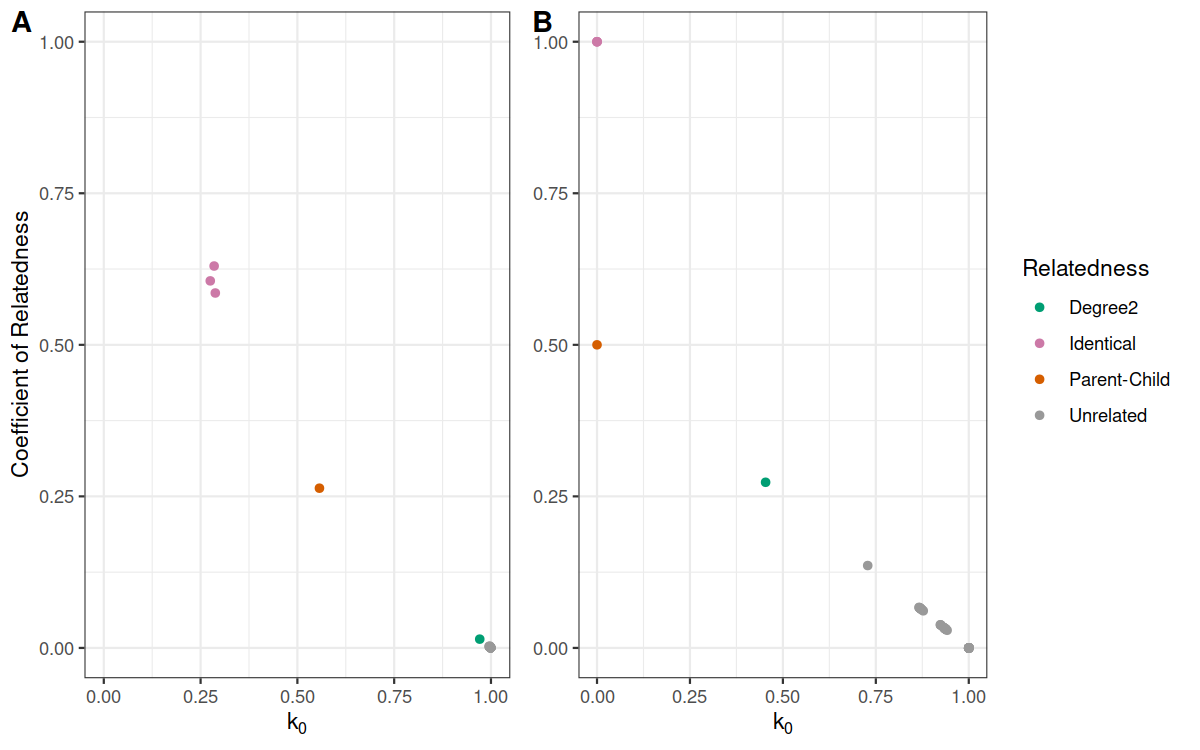
\includegraphics[width=18cm]{supplementary_info/plots/lcPlot.png}
    \caption{Comparison of IBD states estimated for Chagyrskaya specimens using (A) lcMLkin and (B) KIn.
    The relatedness shown with different colors is estimated with and matched with READ and KIn.}
    \label{figS6:Chagyrskaya_ibd}
\end{figure}

This figure shows that it is possible to differentiate between Avuncular and Grandparent-Grandchild pairs.
However, differentiating between Half-siblings may not be possible with our approach. 
*Add 1M windows result
\begin{figure}[h!]
    \centering
    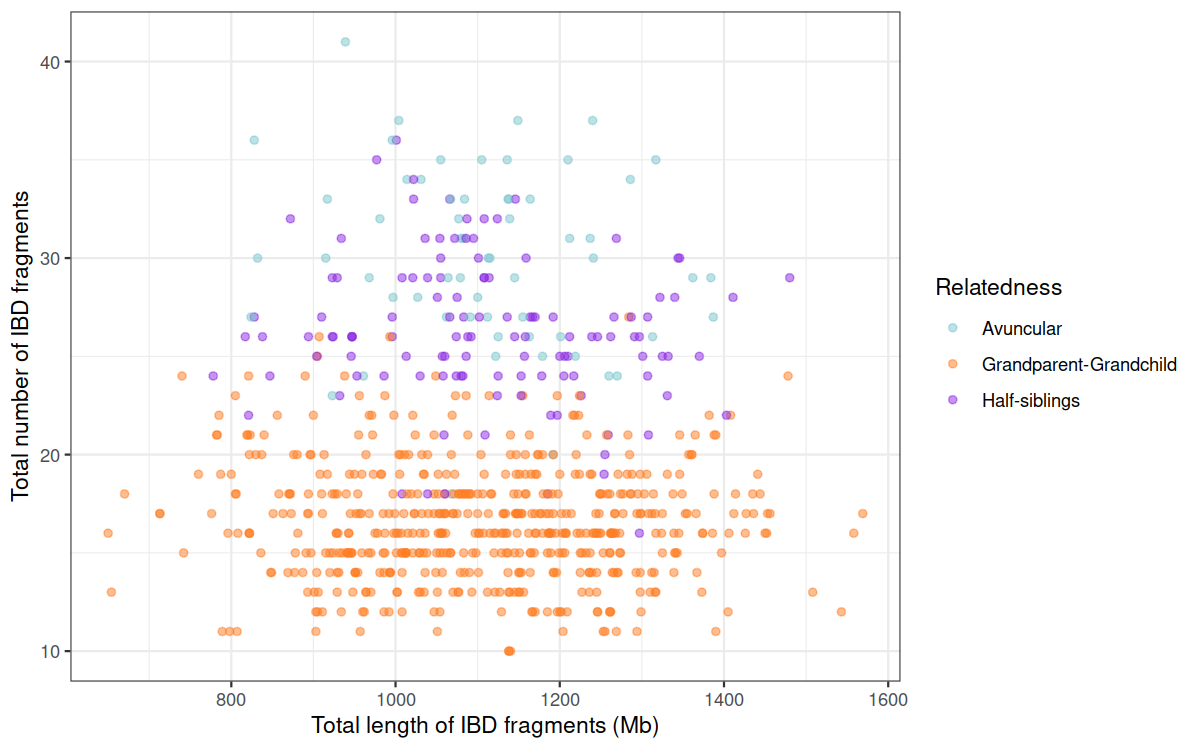
\includegraphics[width=18cm]{supplementary_info/plots/degree2_10Mwin.png}
    \caption{Avuncular and Grandparent-grandchild form different clusters, when total number of IBD fragments are plotted against total length of IBD fragments.}
    \label{figS7:second_degree}
\end{figure}

-READ and KIn differ

-supplementary table2
\begin{figure}[!ht]
    \centering
    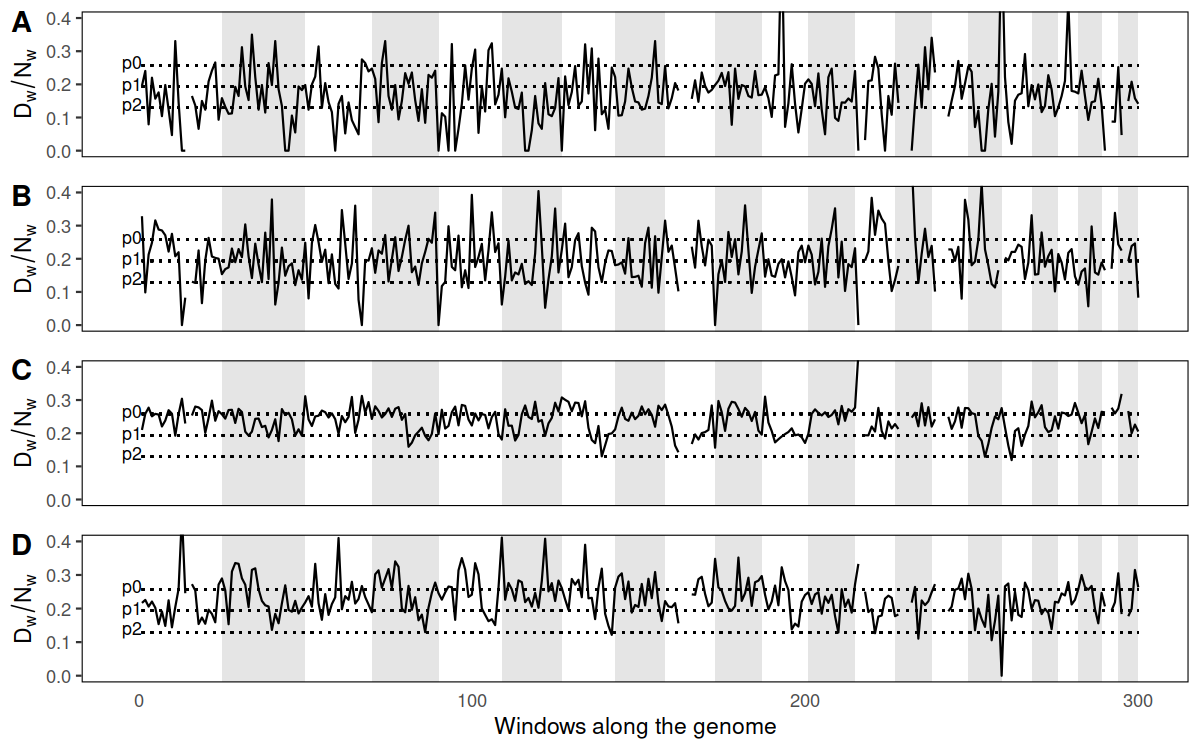
\includegraphics[width=18cm]{supplementary_info/plots/egplot1.png}
    \caption{Plots showing proportion of differences in windows along the genome for some of the pairs of relatives for which KIn differs from READ. (A) AITI62B-OTTM156 (READ estimates Identical individuals, lcMLkin does not have sufficient data, and KIn predicts parent-child. (B) UNTA5867-UNTA5868Sk1 (READ estimates Second Degree, lcMLkin does not have sufficient data, and KIn predicts parent-child). (C) AITI40-AITI72 (READ estimates Unrelated individuals, lcMLkin shows 3rd-5th degree, and KIn predicts 3rd degree.)
    (D) AITI2-AITI55 (READ estimates Unrelated individuals, lcMLkin and KIn predicts predict second degree.)}
    \label{figS8:eg1}
\end{figure}

\begin{figure}[h]
    \centering
    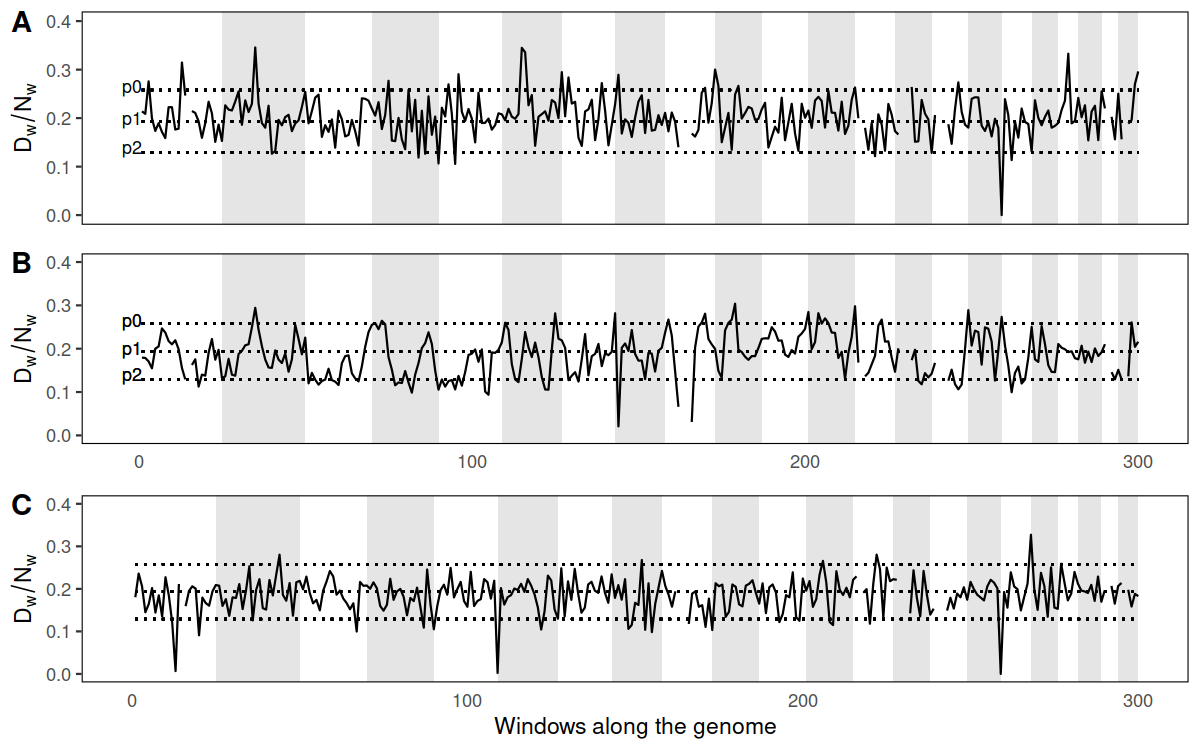
\includegraphics[width=18cm]{supplementary_info/plots/egplot2.png}
    \caption{Plots showing proportion of differences in windows along the genome for some of the pairs of relatives for which KIn differs from lcMLkin. (A) AITI43-AITI55 (READ estimates First degree, lcMLkin predicts siblings, while KIn predicts parent-child. (B) AITI70-AITI72 (READ estimates First degree, lcMLkin predicts parent-child, while KIn predicts siblings.}
    \label{figS9:eg2}
\end{figure}

\bibliographystyle{plain}
\bibliography{references.bib}



\section{Notation summary}
Notation used in the paper:

\begin{itemize}
\item L: Total number of windows
\item w: Index of window
\item $N_w$: Number of sites in w
\item $D_{w}$: Number of pairwise differences in w
\item $Z_w$: Hidden IBD state in window w
\item $i$: States that $Z_w$ can take 
\item $H_w$: ROH state in window w
\item $\omega$ States that $H_w$ can take
\item A: Transition matrix
\item $\pi$: Vector of initial transition probabilities
\item $\theta$: Vector of $\pi$, A, $N_w$ for relatedness HMM
\item $p(Z_w,H_w)$: Expected proportion of differences for given $Z_w$ and $H_w$
\item $x$: Combinations of $i$ and $\omega$ states with unique $p$
\item $\delta$: Over-dispersion parameter
\item $\gamma_{wi}$: posterior probability of $H_w$
\item $h_{\omega w}$: ROH state-probabilities
\item $k_{wx}$: Posterior probability of $x$ in $w$
\item $t$: Threshold on variance of Beta distribution
\item $X$: Random variable from a Beta distribution
\item $y$: Hidden homozygosity states for ROH HMM
\item $Y_w$: Homozygosity state in $w$
\item $\Theta$: Vector of $\pi$, A, $N_w$ for ROH HMM
\item $\Delta_w$: Number of differences within a library 
\item $\rho$: Expected proportion of differences in a library
\item $Gamma$: Posterior probabilities of ROH
\item $\eta$: Overdispersion parameter used in ROH HMM
\item $\mathcal{C}$: Cost function
\item $C_l$: Contamination in library l

\item $c$: Contamination estimate for a library
\item $p_c$: Average proportion of differences between endogenous and contaminating reads
\item $p_e$:Average proportion of differences between endogenous reads
\item $p_a$: Average observed proportion of differences
\item $D_{cor,w}$: Contamination corrected number of differences in $w$
\item $N_{cor,w}$: Contamination corrected number of overlapping sites in $w$
\item $\Xi$: Endogenous read
\item $S_{cor,w}$ $N_{cor,w}$ - $D_{cor,w}$
\item $/mathbf{D_cor}$ Vector of $D_{cor,w}$
\item $G$: Genotype (0,0.5,1)
\item $\lambda$: Expected rate following Poisson distribution
\item $\nu$: Population allele frequency
\item $Lambda$: Log likelihood ratio
\item E: Expectation
\item P: Probability
\end{itemize}



\section{extra}
Many methods exist to estimate relatedness. Most of these work with high coverage, phased data, reference panel, population allele frequency. Other methods that work with low coverage ancient data use likelihoods, but still require 2x coverage.
methods that require a lot of things: PLINK, SNPduo,ERSA,KING,REAP,GRAB,

methods that require low coverage: SEEKIN

mtDNA and Y in relatedness READ paper[15,16,25,16]
snp data better than str when there is damage, low data
excluding related individuals, haak indo europian

READ is a very popular software to estimate relatedness in low coverage ancient DNA. It calculates distance between a pair of individuals using pseudo haploid sequences. These pairwise differences are then normalized by the median of pairwise differences in the population, and compared to the expected pairwise difference given a degree of relatedness. Expected pairwise difference for each case of relatedness is calculated using identity by descent (IBD) probabilities. 

lcMLkin is another widely used method that uses genotype likelihoods to estimate the number of positions at which a pair of individuals have 0/1/2 chromosomes in IBD.  

REAP is a software to estimate relatedness coefficient and IBD prbabilities in admixed populations, accounting for structure. It requires the number of ancestral populations, and a representation of sub population allele frequencies. 

Likelihood estimators:
Milligan BG (2003) Maximum-likelihood estimation of relatedness. Genetics
Anderson AD, Weir BS (2007) A maximum-likelihood method for the estimation of pairwise relatedness in structured populations. Genetics
Choi Y, Wijsman EM, Weir BS (2009) Case-control association testing in the presence of unknown relationships

There are various ways to measure the coefficient of relatedness r. Most methods use the probabilties of IBD to calculate r. There can be, in total 9 modes of identity described by Jacquard (1974), including the cases for 3 IBD probabilities and 3 cases of IBD. Methods assuming outbred population use only the three modes accounting for IBD. Most methods used maximum likelihood approach to estimate r (). Other methods are moment estimators that assume Hardy-Weinberg equilibrium in the population (KING, GCTA).

Discussion

Our contamination correction model requires an estimate of divergence between the contaminating and the target populations. We provide the users an option to provide a file with average pairwise difference between the two populations, or to provide a vcf file with an individual from each population. 
Pipeline has p(diff) instead of pseudohap
Methods
$$\sum_{w} \sum_{I}\sum_\omega \log P(D_{w}|Z_w, H_w)k_{w\omega i}$$



$$P(D_w | N_w, Z_w) = \sum_{k=0}^4 
\underbrace{P(D_w | N_w, k)}_{Betabinomial}
\underbrace{P(k | Z_w, H_w)}_{p matrix}
\underbrace{P(H_w =h)}_{\mathbf{h}_w}
$$

Emission probability in a window depends on both IBD state and ROH state. We obtain posterior probability of one or both individuals being ROH in each window from another HMM described in section 3.2. We calculate the cost function with Betabinomial likelihood in log space for the entire genome as:

The model can be summarised as:

\begin{equation}\label{eq:6}
P(D_w|Z_w,H_w) \sim {\sf Binom}(D_w, N_w, p_{Z,H,w})
\end{equation}

\begin{equation}\label{eq:7}
p_{Z,H,w} \sim {\sf Beta}(\alpha_{Z,H}, \beta_{Z,H})
\end{equation}

Emission probability in a window depends on both IBD state and ROH state. We calculate a cost function as the betabinomial loglikelihood weighted by the posterior probability represented by $\gamma$.
likelihood:
\begin{align}
P(\mathbf{D},\BZ, H|\theta) &= P(\mathbf{D}|\mathbf{Z},H,\theta) P(H |\theta) P(\BZ|\theta)\nonumber\\
&= \prod_{w}  P(D_w|Z_w,  H_w, \theta) \prod_w P(H_w | \theta) \prod_{w} P(Z_w|Z_{w-1}, \theta)] P(Z_0| \theta) 
\end{align}

cost function:
\begin{equation}
    \mathcal{C} = 
       \sum_{w} \sum_{i} \log P(D_{w}|Z_w, H_w)\gamma_{wi}=
    \sum_{w} \sum_{i} 
    \log \left[\sum_{\omega}P(D_{w}|\psi_{i\omega},\delta_{i\omega}) \right] \gamma_{wi}
\end{equation}

\end{document}

